\documentclass[11pt,a4paper,oneside]{report}             % Single-side
%\documentclass[11pt,a4paper,twoside,openright]{report}  % Duplex

%\PassOptionsToPackage{chapternumber=Huordinal}{magyar.ldf}
\usepackage{t1enc}
\usepackage[utf8]{inputenc}
\usepackage{amsmath}
\usepackage{amssymb}
\usepackage{enumerate}
\usepackage[thmmarks]{ntheorem}
\usepackage{graphicx}
\usepackage{epsfig}
\usepackage{listings}
\usepackage{color}
%\usepackage{fancyhdr}
\usepackage{lastpage}
\usepackage{anysize}
\usepackage[magyar]{babel}
\usepackage{sectsty}
\usepackage{setspace}  % Ettol a tablazatok, abrak, labjegyzetek maradnak 1-es sorkozzel!
\usepackage[hang]{caption}
\usepackage{hyperref}
\usepackage{titlesec}
\usepackage{subcaption}
\usepackage{sectsty}
\usepackage{wrapfig}
\usepackage{multirow}
\usepackage{textcomp}
%--------------------------------------------------------------------------------------
% Main variables
%--------------------------------------------------------------------------------------
\newcommand{\vikszerzo}{Papp Dorottya}
\newcommand{\vikkonzulens}{}
\newcommand{\vikcim}{Matematikai statisztika}
\newcommand{\viktanszek}{Hálózati Rendszerek és Szolgáltatások Tanszék}
\newcommand{\vikdoktipus}{Tételsor kidolgozás}
\newcommand{\vikdepartmentr}{}

%--------------------------------------------------------------------------------------
% Page layout setup
%--------------------------------------------------------------------------------------
% we need to redefine the pagestyle plain
% another possibility is to use the body of this command without \fancypagestyle
% and use \pagestyle{fancy} but in that case the special pages
% (like the ToC, the References, and the Chapter pages)remain in plane style

\pagestyle{plain}
%\setlength{\parindent}{0pt} % áttekinthetõbb, angol nyelvû dokumentumokban jellemzõ
%\setlength{\parskip}{8pt plus 3pt minus 3pt} % áttekinthetõbb, angol nyelvû dokumentumokban jellemzõ
\setlength{\parindent}{10pt} % magyar nyelvû dokumentumokban jellemzõ
\setlength{\parskip}{0pt}    % magyar nyelvû dokumentumokban jellemzõ

\marginsize{35mm}{25mm}{15mm}{15mm} % anysize package
\setcounter{secnumdepth}{0}

\chaptertitlefont{\Large}

\setcounter{secnumdepth}{2}
\singlespacing
\frenchspacing

%--------------------------------------------------------------------------------------
%	Setup hyperref package
%--------------------------------------------------------------------------------------
\hypersetup{
    bookmarks=true,            % show bookmarks bar?
    unicode=false,             % non-Latin characters in Acrobat’s bookmarks
    pdftitle={\vikcim},        % title
    pdfauthor={\vikszerzo},    % author
    pdfsubject={\vikdoktipus}, % subject of the document
    pdfcreator={\vikszerzo},   % creator of the document
    pdfproducer={Producer},    % producer of the document
    pdfkeywords={keywords},    % list of keywords
    pdfnewwindow=true,         % links in new window
    colorlinks=true,           % false: boxed links; true: colored links
    linkcolor=black,           % color of internal links
    citecolor=black,           % color of links to bibliography
    filecolor=black,           % color of file links
    urlcolor=black             % color of external links
}

%--------------------------------------------------------------------------------------
% Set up listings
%--------------------------------------------------------------------------------------
\lstset{
	basicstyle=\scriptsize\ttfamily, % print whole listing small
	keywordstyle=\color{black}\bfseries\underbar, % underlined bold black keywords
	identifierstyle=, 					% nothing happens
	commentstyle=\color{white}, % white comments
	stringstyle=\scriptsize\sffamily, 			% typewriter type for strings
	showstringspaces=false,     % no special string spaces
	aboveskip=0pt,
	belowskip=0pt,
	columns=fixed,
	backgroundcolor=\color{lightgray},
} 		
\def\lstlistingname{lista}	

%--------------------------------------------------------------------------------------
%	Some new commands and declarations
%--------------------------------------------------------------------------------------
\newcommand{\code}[1]{{\upshape\ttfamily\scriptsize\indent #1}}

% define references
\newcommand{\figref}[1]{\ref{fig:#1}.}
\renewcommand{\eqref}[1]{(\ref{eq:#1})}
\newcommand{\listref}[1]{\ref{listing:#1}.}
\newcommand{\sectref}[1]{\ref{sect:#1}}
\newcommand{\tabref}[1]{\ref{tab:#1}.}

\DeclareMathOperator*{\argmax}{arg\,max}
%\DeclareMathOperator*[1]{\floor}{arg\,max}
\DeclareMathOperator{\sign}{sgn}
\DeclareMathOperator{\rot}{rot}
\definecolor{lightgray}{rgb}{0.95,0.95,0.95}

\author{\vikszerzo}
\title{\viktitle}
\includeonly{
	titlepage,%
	chapter_1,%
	chapter_2,%
	chapter_3,%
	chapter_4,%
	chapter_5,%
	chapter_6,%
	chapter_7,%
	chapter_8,%
	chapter_9,%
	chapter_10,%
	chapter_11,%
	chapter_12,
	chapter_13
}
%--------------------------------------------------------------------------------------
%	Setup captions
%--------------------------------------------------------------------------------------
\captionsetup[figure]{
%labelsep=none,
%font={footnotesize,it},
%justification=justified,
width=.75\textwidth,
aboveskip=10pt}

\renewcommand{\captionlabelfont}{\small\bf}
\renewcommand{\captionfont}{\footnotesize\it}

%--------------------------------------------------------------------------------------
% Table of contents and the main text
%--------------------------------------------------------------------------------------
\begin{document}
\singlespacing

\pagenumbering{arabic}

\linespread{1.0}
\setlength{\parindent}{0.01em}
\setlength{\parskip}{0.01em}
\titlespacing*{\section}
{0pt}{1.0em plus .1em minus .2em}{.5em plus .2em}
\titlespacing*{\subsection}
{0pt}{1.0ex plus .1em minus .2em}{.5em plus .2em}

%--------------------------------------------------------------------------------------
%	The title page
%--------------------------------------------------------------------------------------
\begin{titlepage}
\begin{center}

\includegraphics[width=60mm,keepaspectratio]{figures/BMElogo.png}\\
\vspace{0.3cm}
\textbf{Budapesti Műszaki és Gazdaságtudományi Egyetem}\\
\textmd{Villamosmérnöki és Informatikai Kar}\\
\textmd{\viktanszek}\\[5cm]

\vspace{0.4cm}
{\huge \bfseries \vikcim}\\[0.8cm]
\vspace{0.5cm}
\textsc{\Large \vikdoktipus}\\[4cm]

\begin{tabular}{cc}
 \makebox[14cm]{\emph{Készítette}}\\
 \makebox[14cm]{\vikszerzo}
\end{tabular}

\vfill
{\large \today}
\end{center}
\end{titlepage}



\tableofcontents\vfill
\setlength{\parskip}{0.5em}
%----------------------------------------------------------------------------
\chapter{Paraméterbecslések}

%----------------------------------------------------------------------------
\section{Alapfogalmak}
%----------------------------------------------------------------------------

A matematikai statisztika alapmodellje:
\begin{itemize}
\item $\mathcal{K}$ a véletlen kísérlet
\item $\Omega$ a lehetséges kimenetelek halmaza
\item $\mathcal{A}$ a megfigyelhető események halmaza
\item $\mathcal{P}$ a lehetéges valószínűségi mértékek halmaza
\end{itemize}
Az elemzésünk célja, hogy $\mathit{P}$-ből kiválasszuk a tényleges valószínűséget, de legalábbis egy jó helyettesítő egyedet.

\emph{Statisztikai minta:} Az $X$ valószínűségi változóval azonos eloszlású, egymással teljesen független $X_1$, $X_2$, ..., $X_n$ valószínűségi változók együttesét statisztikai mintának nevezzük. Egy mintavételkor tulajdonképpen megfigyeljük a $\mathcal{K}$ véletlen kísérletet, azaz megállpítjuk, hogy melyik $\omega \in \Omega$ lehetséges kimenet realizálódott. Az $X_1(\omega)=x_1..., X_n(\omega)=x_n$ szám $n$-est nevezzük a minta realizációjának.

\emph{Statisztika:} Legyen $t_n$ egy $n$-változós valós függvény. A statisztikai minta $t_n(X_1, X_2, ..., X_n)$ függvényét nevezzük statisztikának. A statisztika egy valószínűségi változó, aminek eloszlásfüggvényét a minta eloszlásfüggvényéből lehet kiszámolni. A $T_n = t_n(x_1, x_2, ..., x_n)$ szám a statisztika számolt értéke.

\emph{Paraméter:} Tegyük fel, hogy a minta eloszlásfüggvényének képletét egy $\vartheta$ paraméter konkretizálja, pl. normális eloszlás várható értéke, szórása; binomiális eloszlás paraméterei ($n$ és $k$). Ha ismerjük a paraméter értékét, pontosan meg tudjuk adni az eloszlásfüggvényt $\rightarrow$ cél: adott statisztikai minta segítségével a $\vartheta$ paraméter becslése egy alkalmas statisztikával.

%----------------------------------------------------------------------------
\section{A matematikai statisztika alaptétele (Glivenkó-Cantelli)}
%----------------------------------------------------------------------------

\emph{Empirikus eloszlásfüggvény:}\\
$F_{emp}(x) = 
  \begin{cases}
    0       & \quad \text{ha } x \leq X_1^* \\
    \frac{k}{n}  & \quad \text{ha } X_k^* < x \leq X_{k+1}^*\\
    1		& \quad \text{ha } x>X_n^* \end{cases}
$, ahol $X_i^*$ a rendezett minta $i$-dik eleme

\emph{Glivenkó-Cantelli tétel:} $\mathbf{P}(\lim_{n\rightarrow \infty}\sup_{x\in\mathbb{R}}|F_{emp}(x)-F(x)|=0)=1$, vagyis az empirikus eloszlásfüggvény 1 valószínűséggel, egyenletesen konvergál az eloszlásfüggvényhez. (E miatt a tétel miatt van egyáltalán értelme beszélni a matematikai statisztikáról.)

%----------------------------------------------------------------------------
\section{A jó becslések tulajdonságai}
%----------------------------------------------------------------------------

\emph{Torzítatlanság:} $\mathbf{E}T_n=\vartheta$, vagyis a becslő statisztika pont a becsülendő paraméterérték körül fogja felvenni az értékeit. Indok: egy valószínűségi változó az összes szám körül épp a várható érték körül ingadozik a legkisebb mértékben
	\begin{itemize}
	\item Aszimptotikus torzítatlanság: a torzítatlansági feltétel csak $n \to \infty$ esetében igaz
	\end{itemize}

\emph{Konzisztencia:} $\forall \epsilon >0 \text{-ra } \lim_{n \to \infty}\mathbf{P}(|T_n-\vartheta|>\epsilon) = 0$, vagyis garancia van arra, hogy a minta elemszám növekedtével növekszik a becslés pontosságának valószínűsége
	\begin{itemize}
	\item Erős konzisztencia: torzítatlan becslés, ahol az elemszám növekedtével a szórásnégyzet (variancia, $\mathbf{D}^2T_n$) 0-hoz tart. Az erősen konzisztenc statisztikai becslések egyben konzisztensek is
	\end{itemize}

\emph{Hatásosság:} torzítatlan becslés, melynek varianciája minden más torzítatlan becslés varianciájánál kisebb. Logika: két torzítatlan becslés közül a kisebb szórásnégyzetű a jobb, hiszen kisebb mértékben ingadozik a paraméter körül, vagyis kevesebb megfigyeléssel is jó becslés kapható. Hatásos becslésből egyetlen egy létezik csak, ezt érdemes megkeresni egy adott paraméter-becslési problémához
\begin{itemize}
\item A Cramer-Rao egyenlőtlenség elvi alsó korlátot ad a torzítatlan becslések szórásnégyzeteire. Ha egy statisztikára belátjuk, hogy a szórásnégyzete éppen az alsó korláttal egyenlő, akkor az biztosan a hatásos becslés
\end{itemize}

\emph{Elégségesség:} a mintának $t_n$-re vonatkozó együttes feltétel sűrűségfüggvénye nem tartalmazza a $\vartheta$ paramétert, vagyis a becslés egymaga képes helyettesíteni a mintát, a paraméterre vonatkozóan minden információt magába sűrít
	\begin{itemize}
	\item Rao-Blackwell-Kolmogorov tétel: ha létezik hatásos (legjobb torzítatlan) becslés, akkor elég azt az elégséges becslés függvényei között keresni:\\
	$\exists h(): \mathbf{E}_\vartheta(h(T_n)) = g(\vartheta), \mathbf{\sigma}^2_\vartheta(h(T_n)) \leq \mathbf{\sigma}^2_\vartheta(t_n)$, és $h(T_n) = \mathbf{E}_\vartheta(t_n | T_n)$, ahol $T_n$ a statisztika számított értéke, $g$ a függvény tetszőleges torzítatlan becslése
	\item Az elégségességet a Neymann-Fisher faktorizációs tétellel lehet ellenőrizni:\\
	A $T_n$ statisztika a $\vartheta$ paraméternek akkor és csak akkor elégséges becslése, ha $\exists k : \mathbb{R}^n \rightarrow \mathbb{R}$ és $g:\mathbb{R}^2 \rightarrow \mathbb{R}$ függvények, hogy $\forall (x_1,...,x_n) \in \mathbb{R}^n$ és $\forall \vartheta$-ra\\ $L_\vartheta(x_1,...,x_n)=k(x_1,...x_n) \cdot g(T_n(x1,...,x_n),\vartheta)$, ahol $L_\vartheta(x_1,...,x_n)$ a minta együttes sűrűségfüggvénye
	\end{itemize}


%----------------------------------------------------------------------------
\chapter{Becslési módszerek}

\section{Maximum likelihood becslés}

A módszer alapgondolata, hogy ha egy kísérletnél több esemény is bekövetkezhet, akkor legtöbbször a legnagyobb valószínűségű esetményt fogjuk megfigyelni. Következtetésképp, azért kaptuk azt a mintát, amit, mert ennek a bekövetkezésnek volt a legnagyobb a valószínűsége. Tehát, az összes lehetséges $\vartheta$ paraméter közül vegyük azt, amelynél a kapott realizáció bekövetkezése a maximális! Képletesen: a paraméter maximum likelhood becslése az a $t_n(X_1,X_2, ..., X_n)$ statisztika, melyre $L(x,t_n(\mathbf{x})) = \text{max}_\vartheta L(\mathbf{x}, \vartheta)$ \footnote{$L(\mathbf{x}, \vartheta)$ a likelihood-függvény ($\sum_{i=1}^nP_\vartheta(X_i=x_i)$ diszkrét esetben és $\prod_{i=1}^nf_\vartheta(x_i)$ folytonos esetben.}.

A maximum meghatározásához $L(\mathbf{x}, \vartheta)$ $\vartheta$ szerinti első deriváltjának zérushelyeit keressük. A zérushelyek közül az a maximum, ahol a $L(\mathbf{x}, \vartheta)$ $\vartheta$ szerinti második deriváltja negatív. Megjegyzés: ha $L(\mathbf{x}, \vartheta)$ deriválása túl nehéz, érdemes a logaritmusát venni (log-likehood függvény, $l(\mathbf{x}, \vartheta)$) és azzal számolni. Mivel a logaritmus függvény szigorúan monoton nő, ezért nem torzítja a zérushelyeket. (Többparaméteres esetben paraméterenként vizsgáljuk az első deriváltakat és a Hesse-mátrix alapján döntünk a maximum helyről. Maximum esetén a mátrix diagonális és az első diagonál elem negatív.)

\emph{Cramer-Dugue-tétel:} Tegyük fel, hogy $t_n$ a $\vartheta$ paraméter maximum-likelihood becslése. Legyen a minta sűrűségfüggvénye $f_\vartheta(x)$, $\vartheta \in (a,b)$, ami kielégíti az alábbi feltételeket:
\begin{itemize}
\item létezik $ln \big(f_\vartheta(x) \big)$ első 3 deriváltja,
\item létezik $H_1(x), H_2(x), H_3(x)$, amelyek az indexnek megfelelő deriváltak abszolút értékeinek felső becslései, $H_1(x)$ és $H_2(x)$ teljes számegyenesen vett integráltjai léteznek, $H_3(x) \cdot f_\vartheta(x)$ teljes számegyenesen vett integrálja felülről korlátos és
\item $0<I_1(\vartheta)=\int_{- \infty}^{\infty} \big(\frac{\partial ln f_\vartheta(x)}{\partial \vartheta}\big)^2 \cdot f_\vartheta(x) dx < \infty$
\end{itemize}
Ekkor $t_n$ a $\vartheta$ paraméter konzisztens becslése és aszimptotikusan normális eloszlású. (Pluszban: ha létezik elégséges statisztika, akkor éppen azt adja meg, bár ez a tulajdonság nem tartozik a tételhez.)

\section{A momentumok módszere}

Legyen adott a valószínűségi mértékek egy tere és az $X_1, X_2, ..., X_n$ statisztikai minta. Tegyük fel, hogy létezik az első $k$ momentum ($m_j = \mathbf{E}_\mathbf{\vartheta}X_i^j$), és $\exists g_j^{-1}(m_1, m_2, ..., m_k) = \vartheta_j$. Tekintsük az $\hat{m}_j=\frac{1}{n}\sum_{i=1}^nX_i^j$ empirikus momentum statisztikákat. Ekkor az $m_j = g_j^{-1}(\hat{m}_1,..., \hat{m}_k)$ statisztikák a $\vartheta_j$ paraméterek momentumos becslései.

\section{Normális eloszlásból származtatott eloszlások}

\begin{table}[h]
\centering
\begin{tabular}{|p{2.7cm}|p{5.8cm}|p{5cm}|}
\hline
Név & Sűrűségfüggvény & Származtatása
\\ \hline
$\chi^2$-eloszlás & $ \frac{1}{2^{n/2}\Gamma(n/2)} \cdot e^{-x/2} \cdot x^{(n/2)-1}$ & \multirow{3}{5cm}{standard normális, független változók négyzetösszege $\chi^2_n$-eloszlást követ} \\
&  $ x>0 $ & \\
 & $\Gamma(s) = \int_0^\infty e^{-t} \cdot t^{s-1} dt$ &
\\ \hline
Student-eloszlás & $\frac{\Gamma(\frac{n+1}{2})}{\Gamma(1/2)\Gamma(n/2)} \cdot 1/\sqrt{n} \cdot \Big(\frac{1}{1+x^2/n} \Big)^{\frac{n+1}{2}}$ $x \in \mathbb{R}$ & standard normális, független valószínűségi változók esetén $\frac{Y}{\sqrt{\frac{\sum_{i=1}^{n}X_i^2}{n}}}$ $t_n$-eloszlást követ
\\ \hline
Fisher-eloszlás & $\frac{\Gamma(\frac{n+k}{2})}{\Gamma(n)\Gamma(k)} \cdot x^{(k/2)-1} \cdot \Big(k+nx \Big)^{-\frac{k+n}{2}}$ $x > 0$ & $X \in \chi^2_n$, $Y \in \chi^2_k$ és független $X$-től, akkor $\frac{X/n}{Y/k}$ $F_{n,k}$-eloszlást követ
\\ \hline
\end{tabular}
\end{table}

\emph{Lukács-tétel:} Legyenek $X_1, X_2,...X_n \in N(m,D)$ teljesen függetlenek. Ekkor
\begin{itemize}
\item az átlag $N(m,\frac{D}{\sqrt{n}})$ eloszlást követ
\item $\frac{ns_n^2}{D^2} \in \chi_{n-1}^2$
\item az átlag és $s_n^2$ függetlenek
\end{itemize} 

\section{Konfidencia intervallumok}

Eddig az ismeretlen paramétervektort a minta egy függvényével, azaz egyetlen statisztikával próbáltuk meg közelíteni. Konkrét realizációnál tehát, a paramétertér egy pontját egy másik ponttal becsüljük (\emph{pontbecslés}).

Folytonos eloszlásoknál azonban annak valószínősége, hogy a valószínőségi változó az értékkészletének éppen egy tetszőlegesen kiválasztott pontját fogja felvenni, nulla. Tehát folytonos esetben nulla annak valószínősége, hogy éppen a paramétert találtuk el a becsléssel. Az intervallumbecsléseknél a mintából készített tartományokat definiálunk, amely tartományok nagy valószínőséggel lefedik a kérdéses paraméterpontot.

Legyen adott a valószínűségi mértékek egy tere és az $X_1, X_2, ..., X_n$ statisztikai minta. Legyen $0<\epsilon<1$ rögzített. A $\vartheta$ paraméterhez megadhatunk egy legalább $1-\epsilon$ szignifikanciaszintű konfidencia-intervallumot, ha $t_1(X_1, X_2, ..., X_n)$ és $t_2(X_1, X_2, ..., X_n)$ olyan statisztikák, hogy:
$\mathbf{P}_\vartheta(t_1(X_1, X_2, ..., X_n) \leq \vartheta \leq t_2(X_1, X_2, ..., X_n)) \geq 1-\epsilon$ mindig igaz.


%----------------------------------------------------------------------------
\chapter{Statisztikai hipotézisvizsgálat}

\section{Hipotézisek, próbastatisztika, kritikus tartomány}

Adott a $\mathcal{K}$ véletlen kísérlet, az $\Omega$ eseménytér,  a lehetséges valószínűségek halmaza $\mathcal{P}$ és a felette értelmezett $\mathbf{P}$ Kolmogorov-féle valószínűségi mező. Tegyük fel, hogy $\mathcal{P}$ két diszjunkt halmazra bontható: $\mathcal{P}_0$ és $\mathcal{P}_1$. Statisztikai próbát akarunk kidolgozni annak eldöntésére, hogy $H_0:\mathbf{P}\in\mathcal{P}_0$ \emph{nullhipotézis} igaz-e. Ha úgy kell döntenünk, hogy a null hipotézis nem igaz, akkor automatikusan a $H_1:\mathbf{P}\in\mathcal{P}_1$ \emph{alternatív hipotézist} fogjuk elfogadni. A döntéshez szignifikancia szintet rendelünk, amivel jellemezzük, hogy mennyire erős a döntésünk.

\emph{Kritikus érték:} $\forall \epsilon \in (0,1)$ számhoz megadhatók $K_1(\epsilon) < K_2(\epsilon)$ kritikus értékek úgy, hogy $\mathbf{P}_\nu(K_1(\epsilon)< T_n < K_2(\epsilon)) \geq 1-\epsilon$, $\nu \in \Theta_0$.

\emph{Elfogadási tartomány:} $\mathcal{X}_e = \{\underline{x} \in \mathbb{R}^n : K_1(\epsilon)< T_n < K_2(\epsilon)\}$. Ha $\underline{x} \in \mathcal{X}_e$, akkor a $H_0$ hipotézist elfogadjuk a $\epsilon$ szignifikancia-szinten ($\underline{x}$ a mintarealizáció).

\emph{Kritikus tartomány:} $\mathcal{X}_k = \mathbb{R}^n \setminus \mathcal{X}_e$


\section{Első - és másodfajú hibavalószínűség}

A döntésünk nem lesz minden esetben helyes, elképzelhető, hogy hibásan döntünk.


\begin{figure}[h]
  \caption{Hibafajták}
  \centering
  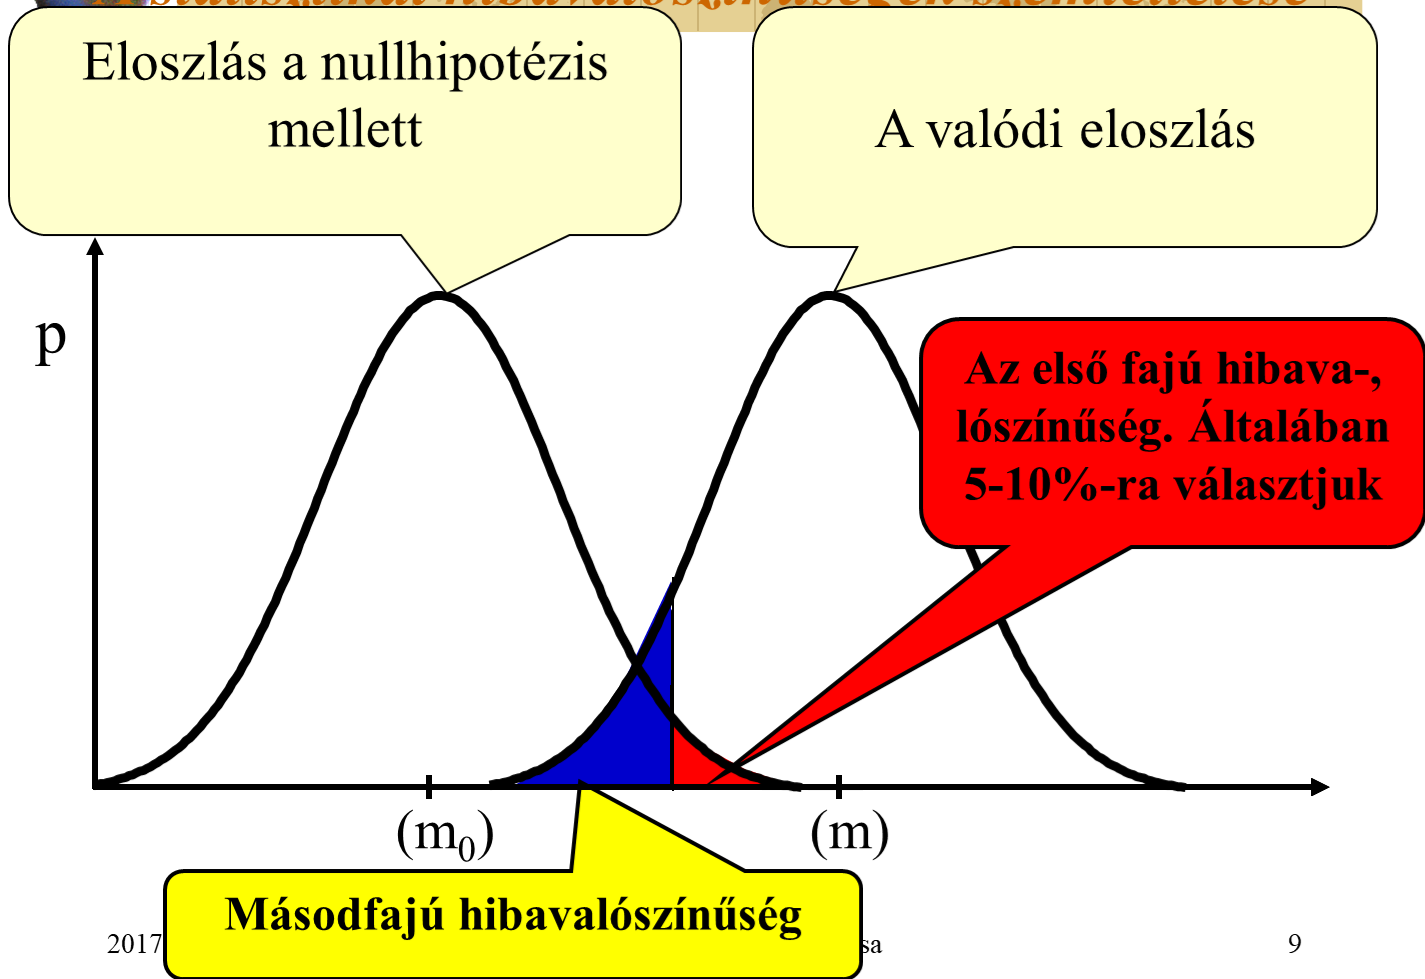
\includegraphics[width=0.7\textwidth]{figures/hibafajtak.png}
\end{figure}


\emph{Elsőfajú hiba:} $H_1$-et fogadjuk el, minközben $H_0$ igaz. Ennek értékét tudjuk befolyásolni, általában 5-10\%-ra választjuk.

\emph{Másodfajú hiba:} $H_0$-t fogadjuk el, miközben $H_1$ az igaz. A másodfajú hiba értékét nehéz megállapítani.

A két hibafajta között trade-offot kell találni, ha az egyiket csökkentjük, a másik nőni fog. A hibavalószínűségeket csak úgy tudjuk csökkenteni, ha növeljük a mintaelemszámot (mivel így a sűrűségfüggvények szórása csökken)

További vonatkozó tételek:
\begin{itemize}
\item \emph{Neyman-Pearson fundamentális lemma:}  Adottak a minta sűrűségfüggvényei $\mathbf{P}_0$ és $\mathbf{P}_1$ valószínűségi mértékekre ($f_0$ és $f_1$), melyeknek együttes sűrűségfüggvényei $L_0$ és $L_1$. Amennyiben dönteni szeretnénk a null hipotézisről az alternatív hipotézissel szemben, akkor
\begin{itemize}
\item tetszőleges $0<\epsilon<1$ esetén $\exists c_0 >0$ és $0 < \tau < 1$ szám, amivel a \\
$\Phi(x) = 
  \begin{cases}
    1       & \quad \text{ha } L_1(x) > c_0L_0(x) \\
    \tau    & \quad \text{ha } L_1(x) = c_0L_0(x)\\
    0		& \quad \text{ha } L_1(x) < c_0L_0(x)
  \end{cases}
$
\\döntésfüggvény olyan véletlenített próbához tartozik, aminek $\epsilon$ a terjedelme
\item az előbb definiált próba egyenletesen legjobb próba
\item ha $\Phi*$ egy $\epsilon$ terjedelmű legjobb próba, akkor \\$\mathbf{P}_0(\Phi(x) = \Phi*(x))=\mathbf{P}_1(\Phi(x) = \Phi*(x))=1$
\end{itemize}
E lemma segítségével lehet rögzített elsőfajú hibavalószínűséghez a lehető legkisebbb másodfajú hibavalószínűségű próbát megkonstruálni

\item \emph{Stein-lemma:} Adottak a minta sűrűségfüggvényei $\mathbf{P}_0$ és $\mathbf{P}_1$ esetén, melyeknek relatív entrópiája $| \mathbf{D} (f_0 || f_1)| = \Big| \mathbf{E}_{\mathbf{P}_0}log_2\frac{f_0(X_1)}{f_1(X_1)} \Big|$ véges. Legyen $\alpha_n$ az elsőfajú hibavalószínűség, $\beta_n$ pedig a másodfajú hibavalószínűség. Legyen $\beta_{n,\epsilon}$, $0<\epsilon<1/2$ a legfeljebb $\epsilon$ terjedelmű próbák esetén a minimális másodfajú hibavalószínűség.\\Ekkor $lim_{n\rightarrow\infty}log_2\beta_{n,\epsilon} = - \mathbf{D} (f_0 || f_1)$
\end{itemize}

\section{Erőfüggvény, próba konzisztenciája, torzítatlansága, ereje}

\emph{Erőfüggvény: } $E(\epsilon, n, \mathbf{P}) = \mathbf{P}((X_1,X_2,...X_n)^T \in \mathcal{X}_k)$, $\mathbf{P} \in \mathcal{P}_1$, $0<\epsilon<1$, $n \in \mathbb{N}$

Próba \emph{ereje:} $\sup_{\forall \mathbf{P} \in \mathcal{P}}\mathbf{P}((X_1,X_2,...X_n)^T \in \mathcal{X}_k)$

Próba \emph{torzítatlansága:} 
\\$\mathbf{P}((X_1,X_2,...X_n)^T \in \mathcal{X}_k) \leq \epsilon$, $\forall \mathbf{P} \in \mathcal{P}_0$-ból következik, hogy \\$\mathbf{P}((X_1,X_2,...X_n)^T \in \mathcal{X}_k) \geq \epsilon$, $\forall \mathbf{P} \in \mathcal{P}_1$, $0<\epsilon<1$, vagyis ha a nullhipotézis nem áll fenn, akkor nagyobb valószínűséggel utasítjuk el, mint amikor fennáll.

Próba \emph{konzisztenciája:} $\lim_{n\rightarrow\infty}E(\epsilon, n, \mathbf{P}) = 1$, $\forall \mathbf{P} \in \mathcal{P}_1$, $0<\epsilon<1$
%----------------------------------------------------------------------------
\chapter{Próbák}

\section{Paraméteres próbák}

Paraméteres próbák esetén $\mathcal{P} = \{ \mathbf{P}_\vartheta : \vartheta \in \Theta\}$, $\Theta = \Theta_0 \cup \Theta_1$, $\Theta_0 \cap \Theta_1 = \emptyset$, ahol $\Theta$ a paramétertér. A nullhiptézis, hogy $\vartheta \in \Theta_0$, az alternatív hipotézis pedig, hogy $\vartheta \in \Theta_1$. Feltételezzük, hogy a minta normális eloszlást követ, a nullhipotézist pedig a normális eloszlás paramétereivel kapcsolatban fogalmazzuk meg.\footnote{A vizsgán használhattuk a képletgyűjteményt, így a képleteket nem gépeltem le.} Akkor döntünk a nullhipotézis mellett, ha a számolt próbastatisztika kisebb a kritikus értéknél.

\begin{table}[h]
\centering
\caption{Paraméteres próbák}
\label{tab:param}
\begin{tabular}{|p{2,5cm}|p{5cm}|p{3cm}|p{3cm}|}
\hline
\textbf{Próba neve}            & \textbf{Feltétel}                                                             & Paraméter & Döntés                   \\ \hline
egymintás u-próba              & szórás ismert & várhetó érték & $|u_{proba}| < K_{krit}$ \\ \hline
kétmintás u-próba              & független statisztikai minták, szórásaik ismertek & várható érték & $|u_{proba}| < K_{krit}$ \\ \hline
egymintás t-próba              & szórás nem ismert & várható érték &  $|t_{proba}| < K_{krit}$ \\ \hline
független kétmintás t-próba    & minták függetlenek, szórásai egyenlőeknek tekintendők ($\rightarrow$ F-próba) & várható érték &  $|t_{proba}| < K_{krit}$ \\ \hline
összetartozó kétmintás t-próba & & várható érték &  $|t_{proba}| < K_{krit}$ \\ \hline
Welch-próba                    & független, normális eloszlású minták, eltérő szórással (amik nem ismertek) & várható érték &  $|W_{proba}| < K_{krit}$ \\ \hline
F-próba                        & független, normális eloszlású minták, szórás nem ismert & szórás &  tört $\in F_{n-1,m-1}$   \\ \hline
Bartlett-próba                        &  & szórás & $W \in \chi^2_{p-1}$   \\ \hline
\end{tabular}
\end{table}

\emph{Egymintás u-próba:} a normális eloszlású mintának ismerjük a szórását és arra vagyunk kiváncsiak, hogy a várható értéke $m_0$-e. A nullhipotézis ellenőrzéséhez első lépésben kiszámoljuk a próbastatisztika abszolútértékét. Második lépésben a kritikus értéket kell meghatároznunk: $\mathbf{P}(|N(0,1)| < u_{krit})= \mathbf{P}(-u_{krit} < N(0,1) < u_{krit}) = \Phi(u_{krit}) - \Phi(-u_{krit}) = 2 \Phi(u_{krit}) -1 = 1-\epsilon$, vagyis $\Phi(u_{krit}) = 1-\epsilon/2$. A kritikus értéket ez alapján a megfelelő táblázatból olvashatjuk ki. Az egymintás u-próba torzítatlan és konzisztens, ráadásul egyenletesen legjobb próba is.

\emph{Kétmintás u-próba:} adott két, egymástól független statisztikai minta, amelyek normális eloszlást követnek és a szórásaik ismertek. Nullhipotézisünk, hogy a két minta várható értéke megegyezik. Kétmintás esetben a döntéshez majdnem ugyanazokat a lépéseket kell elvégeznünk, mint egymintás esetben, csak a próbastatisztikát számoljuk másként (lásd képletgyűjtemény).

\emph{Egymintás t-próba:} normális eloszlású mintának nem ismerjük a szórását, de feltételezzük, hogy várható értéke $m_0$. Hogy a feltételezéstől döntsünk, ki kell számolnunk a próbastatisztika értékét, ami $t_{n-1}$ eloszlást követ, ha igaz a nullhipotézis. A kritikus értéket a $\mathbf{P}(|t_{n-1}| < t_{krit}) = 1-\epsilon$ összefüggésből kapjuk.

\emph{Független mintás t-próba} esetén először meg kell győződnünk arról, hogy a minták szórása egyenlőnek tekinthető-e. Ezt $F$-próbával tehetjük meg. Ha az F-próba sikeres, akkor elvégezhetjük a független mintás t-próbát. Nullhipotézisünk, hogy a minták várható értékei egyenlőek. Először kiszámoljuk a próbastatisztika abszolútértékét, ami $t_{n+m-2}$ eloszlást követ, ha a nullhipotézis igaz, majd ezt hasonlítjuk össze a kritikus értékkel a megfelelő táblázatból. 

\emph{Összetartozó mintás t-próba:} nullhipotézisünk, hogy a minták várható értékei egyenlőek. Ellenőrzéshez kiszámoljuk a próbastatisztika abszolútértékét, ami $t_{2n-2}$ eloszlást követ, ha igaz a nullhipotézis, és ezt hasonlítjuk össze a próbastatisztika értékével.

\emph{Welch-próba:} független mintás t-próbát akartunk, de az $F$-próba sikertelen volt, vagyis a szórások nem tekinthetőek egyenlőnek. Ilyenkor Welch-próbával dönthetünk arról, hogy a várható értékek megegyeznek-e. A próbastatisztika közelítőleg $t_f$ eloszlást követ, ha igaz a nullhipotézis, ahol $f$-et külön számolni kell a képletgyűjteményben megadottak szerint. Ha megvan $f$, táblázatból kinézhetjük a kritikus értéket és meghozhatjuk a döntést.

\emph{$F$-próba:} két független mintáról eldönthetjük vele, hogy a minták szórásai egyenlőnek tekinthetőek-e. A próbastatisztika $F_{n-1,m-1}$ eloszlást követ, ha igaz a nullhipotézis, a képletben $s^*_{x,m}$ az $X$ minta empirikus szórásnégyzete:  $s^*_{x,m} = \frac{1}{n-1} \Sigma_{i=1}^n(X_i - \bar{X_n})^2$.

A \emph{Bartlett-próba} az $F$-próba általánosítása, nem két, hanem $p$ független mintáról dönti el, hogy szórásaik egyenlőnek tekinthetőek-e. A próbastatisztika $\chi^2_{p-1}$ eloszlást követ, ha igaz a nullhipotézis, vagyis abból a táblázatból kell nézni a kritikus értéket.

\section{Nemparaméteres próbák}

Ha a statisztikai minta eloszlását nem tekintjük eleve ismernek, akkor nemparaméteres próbákról beszélünk. Ilyenkor az előzetes felvetéseink nagyon általánosak, de természetesek, pl. szórás véges, eloszlás folytonos, stb. Mivel kevesebb feltételt követelünk meg kiinduláskor, a következtetések levonásához nagyobb elemszámú mintára lesz szükségünk.

\subsection{Tiszta illeszkedésviszgálat}

Nullhipotézisünk, hogy az elemzett változó eloszlása megegyezik a hipotetikussal. A nullhipotézisről dönthetünk \emph{$\chi^2$-próbával}. Adjuk meg a minta értékkészletének egy tetszőleges $r$ diszjunkt intervallumból álló felosztását. Tudjuk, hogy mekkora egy-egy esemény bekövetkezésének valószínűsége a hipotetikus eloszlás esetén ($\nu_i$) és mekkora lett a mintánk esetén ($p_i$). Ha a nullhipotézis igaz, akkor $\Sigma^r_{i=2} \frac{(\nu_i - np_i)^2}{npi}$ aszimptotikusan $r-1$ szabadságfokú $\chi^2$ eloszlást követ, $n$ a minta elemszáma. A kritikus értéket a megfelelő táblázatból kapjuk.
%----------------------------------------------------------------------------
\chapter{Szórásanalízis aka ANOVA}

A célünk kideríteni, hogy van-e hatása a független változóknak a függő változóra illetve, hogy ez a hatás egyforma vagy különböző. A hatás, kapcsolat függvényszerű feltárása akkor sem cél, ha a független változók kvantitatívek. A szórásanalízis megelőzi a regressziós vizsgálatokat, megadja, hogy van-e értelme keresni az összefüggés jellegét. Alapfogalmak:
\begin{itemize}
\item \emph{Faktor:} a vizsgálatba bevont változók
\begin{itemize}
\item Kvantitatív faktor: numerikus vagy intervallum skálájú
\item Kvalitatív faktor: nem kvantitatív
\end{itemize}
\item \emph{Faktor szint:} a faktor értékkészletének egy eleme, ezen beállítások mellett figyeljük meg a függő változót
\begin{itemize}
\item Véletlen faktor: nem tudjuk előre garantálni, hogy milyen értéket vesz fel
\item Beállított faktor: a felvett értékeket előre be tudjuk állítani
\end{itemize}
\item \emph{Interakció:} az egyes faktorok között feltételezett kapcsolat
\item \emph{Kezelés:} egyfaktoros esetben a faktor szintje, többfaktoros esetben a figyelembe vett faktorok szintjeiből előálló kombinációk
\end{itemize}

A modelleket a faktorok száma szerint csoportosítjuk, így beszélhetünk egy-, két-, háromfaktoros modellekről stb. Bizonyos kérdéseket csak többfaktorok modellekben tehetünk fel (pl. interakció kérdése).

\section{Fisher-Cohran tételek}

\emph{Addíciós tétel:} Ha $Q_1, Q_2, …, Q_k$ teljesen független rendre $n_1, n_2, …, n_k$ szabadságfokú $a>0$ paraméterű $\chi^2$-eloszlású változók, akkor a $Q= Q_1+ Q_2+ …+ Q_k$ szintén $\chi^2$-eloszlású lesz $n= n_1+ n_2+ …+n_k$ szabadságfokkal és $a>0$ paraméterrel.

\emph{Partíciós tétel:} Legyenek $X_1, X_2,...,X_n$ teljesen független, $0$ várható értékű és $a$ varianciájú normális eloszlású változók, $Q_j=X^T\mathbf{\underline{A}}_jX  (j=1,2,…, k)$ kvadratikus alakok, ahol $rank(A_i)=n_i$. Tegyük fel, hogy $n= n_1+ n_2+ …+n_k$ és $Q_1+ Q_2+ …+ Q_k = X_1^2+X_2^2+ …+X_n^2$. Akkor a $Q_1, Q_2, …, Q_k$ kifejezések rendre $n_1, n_2, …, n_k$ szabadságfokú, $a>0$ paraméterű, teljesen független $\chi^2$-eloszlású változók.

\section{Kísérleti elrendezések}

\emph{Hierarchikus osztályozás:} a faktorok hierarchiában vannak és egy faktor összes szintje a felette álló faktor egy szintjéhez kapcsolódik. Ilyen kísérleti beállítást követünk, amikor $p$ osztály tanulóinak tudását akarjuk összehasonlítani, $r$ különböző tantárgy számonkérésével.

\emph{Keresztosztályozás:} Az $A$ és $B$ faktor szintjeinek minden párosításához veszünk egy- vagy többelemű mintát. Kettőnél több faktor esetén azon kezelés kombinációhoz veszünk mintát, ahol $k$ a faktorok száma.

\emph{Nem teljes kísérleti elrendezések:} olyankor alkalmazandó, amikor egy vizsgálandó faktor mellett más, nem kívánt, de számontartott hatás is fellép és azokat ki akarjuk küszöbölni, pl. a latin négyzetek módszerével. Tegyük fel, hogy a célváltozónkkal három kategóriaváltozó van kapcsolatban, mindegyik $r>1$ szinttel:
\begin{itemize}
\item \emph{Véletlen blokkok módszere:} $C$ faktor hatását úgy elimináljuk, hogy a $B$ faktor minden szintjéhez az $A$ faktor szintjeinek egy véletlen permutációját rendeljük. Ilyenkor $r^3$ kezelésre van szükség
\item \emph{Latin négyzete módszere:} $r^2$ kezelés is elég a döntéshez az alábbi szisztéma szerint:

\begin{table}[h]
\centering
\begin{tabular}{|l|l|l|l|l|}
\hline
 & $A_1$ & $A_2$ & $...$ & $A_p$
\\ \hline
$B_1$ & $C_{11}$ & $C_{12}$ & $...$ & $C_{1p}$
\\ \hline
$B_2$ & $C_{21}$ & $C_{22}$ & $...$ & $C_{2p}$
\\ \hline
... & ...& ...&...& ...
\\ \hline
$B_r$ & $C_{r1}$ & $C_{r2}$ & $...$ & $C_{rp}$
\\ \hline
\end{tabular}
\end{table}

A módszer feltételezi, hogy a faktorok közötti interakciók nem jelentősek. Alkalmazásának feltételei:
\begin{enumerate}
\item Minden kezeléshez tartozó mintának követnie kell a normális eloszlást
\item Minták szórásnégyzeteinek meg kell egyezniük
\item Mintáknak függetleneknek kell lenniük
\end{enumerate}

Tekintsünk egy $H=(h_{ij})$ $r$x$r$-es latin négyzetet (mátrix, aminek minden sora és oszlopa $1,...,r$ véletlen permutációja)! A három faktor minden $(i, j, h_{ij})$ szintbeállítása mellett figyeljük meg a célváltozó értékét ($X_{ijh}$)! Feltesszük, hogy a $X_{ijh}$ változók teljesen független normális eloszlásúak és $\mathbf{E}X_{ijh}=f_h+b_i+c_j$, $\mathbf{\sigma}X_{ijh}=\sigma$, vagyis célváltozó várható értékére mindhárom faktor additív taggal van hatással.

$H_0$: a harmadik faktor szintjei nincsenek hatással a célváltozóra, vagy $f_j$ mindenhol azonos.

A döntéshez a faktorok szintjeihez tartozó átlagok és a minta teljes átlagának négyzetes eltéréseit kell vizsgálni, valamit ki kell számolni a véletlen ingadozásokat kifejező négyzetes eltérést is. Amennyiben igaz a nullhipotézis, akkor a \\$\frac{\text{harmadik faktorhoz tartozó eltérések négyzetösszege}}{\text{véletlen ingadozásokat kifejező négyzetes eltérés}}(r-2)$ próbastatisztika \\$F_{(r-1),(r-1)(r-2)}$-eloszlást követ.

\end{itemize}

\pagebreak

\section{Egyszeres osztályozás}

Egy $X$ normális eloszlású változónak egyetlen $L$ szintű faktorváltozóval való kapcsolatát vizsgáljuk (one-way-ANOVA). Az $X$-re vett $n$ elemű mintát a faktor szintjei szerint $L$ csoportba soroljuk.

$H_0$: az $L$ db minta átlagai között nincs különbség

Amennyiben igaz a nullhipotézis, akkor a $\frac{\frac{\Sigma^L_{i=1}n_i \big(\bar{x}^{(i)} - \bar{x} \big)^2}{L-1}}{\frac{\Sigma^L_{i=1}n_i \big (x^{(i)}_j - \bar{x}^{(i)} \big)^2}{n-L}}$ statisztika\\ $F_{(L-1),(n-L)}$-eloszlású lesz. Ha a nullhipotézist el kell vetni, akkor az eltérések nagyságát Student próbával lehet megbecsülni.

\section{Kétszeres osztályozás}

Ha egy folytonos függőváltozó, és két nominális faktorváltozó adott, kétszeres osztályozásról beszélünk. Tegyük fel hogy az egyik faktor értékei az $1, 2, ..., L$ a másik faktor értékei az $1, 2, ..., K$ közül valók. Így a mintát összesen $K$x$L$ részhalmazra bonthatjuk. Feltesszük, hogy a minták normális eloszlásúak és a szórásaik ismeretlenek, de azonos értékűek.

Ha a két nominális faktorváltozó között nincs interakció, akkor feltesszük a $(j,k)$ cella elméleti várhatóértéke $\mu_{j,k} = a_j+g_k$ alakú, ahol az első tag az első faktor $j$ szintjéből, a második tag pedig a második faktor $k$ szintjéből eredő tag.

$H_0$: Az első faktor szintjeihez ugyanakkora hatás tartozik minden cellában

Amennyiben igaz a nullhipotézis, akkor a
$\frac{\frac{L \cdot \Sigma^L_{i=1}n_i \big(\bar{x}_i - \bar{x} \big)^2}{L-1}}{\frac{\text{véletlen ingadozásokat mérő négyzetösszeg}}{(L-1)(K-1)}}$
statisztika\\ $F_{(L-1),(L-1)(K-1)}$ eloszlást követ. Vagyis, ha a nullhipotézist elfogadjuk, akkor az első faktornak nincsen hatása a célváltozóra.

Ezzel az eljárással a második faktor hatását is tesztelhetjük, csak akkor a próbastatisztikában a felsző tört számlálójába $K \cdot \Sigma^K_{j=1}n_i \big(\bar{x}_j - \bar{x} \big)^2$ (a második faktor magyarázta négyzetösszeg) kerül.

Ha interakciót is feltételezünk a faktorok között, akkor a $(j,k)$ cella elméleti várhatóértéke $\mu_{j,k} = \mu + a_j+g_k + c_{i,j}$ alakú, ahol $c_{i,j}$ fejezi ki, hogy a hatások erősítik vagy gyengítik egymást. A módszer alkalmas egyidejűleg három hipotézis ellenőrzésére is:
\begin{enumerate}
\item Az első faktornak minden cellában ugyanakkora a hatása
\item A második faktornak minden cellában ugyanakkor a hatása
\item $c_{i,j}=0$ minden cellában
\end{enumerate}

A nullhipotézisek ellenőrzéséhez itt is az átlagtól való eltérés négyzetösszegeit kell számolunk: az első és második faktor magyarázta eltérések négyzetösszegei, az interakcióval magyarázott eltérés négyzetösszege és a csoportokon belüli ingadozásokat mérő véletlen hibatag. A próbastatisztikáknak igaz nullhipotézisek esetén $F$-eloszlást kell követnie.

%----------------------------------------------------------------------------
\chapter{Nemparaméteres próbák}

Ha a statisztikai minta eloszlását nem tekintjük eleve ismernek, akkor nemparaméteres próbákról beszélünk. Ilyenkor az előzetes felvetéseink nagyon általánosak, de természetesek, pl. szórás véges, eloszlás folytonos, stb. Mivel kevesebb feltételt követelünk meg kiinduláskor, a következtetések levonásához nagyonn elemszámú mintákra lesz szükségünk.

\section{Függetlenségvizsgálat}

Függetlenségvizsgálat esetén a nullhipotézisünk, hogy az elemzett változók függetlenek. A nullhipotéziról $\chi^2$-próbával dönthetünk, ahol $n$ elemszámú, kétdimenziós statisztikai mintánk van $(X_1,Y_1), ... , (X_n,Y_n)$. Mindkét minta értékeiből halmazokat készítünk úgy, hogy $I_k = [x_{k-1}, x_k)$ és $J_k = [y_{k-1}, y_k)$. Jelölje $V_{ij}$ azon mintaelemek számát, ahol $(X_i,Y_j) \in I_i \times J_j$, $p_{ij} = \mathbf{P}(X_k \in I_i, Y_k \in J_j)$. Becsléses illeszkedésvizsgálatot hajtunk végre, ahol a becsült paraméterek száma $r+s-2$, a próbastatisztikát a képletgyűjtemény alapján számoljuk. Ha a nullhipotézis igaz, akkor a próbastatisztika eloszlása $(r-1)(s-1)$ szabadságfokó $\chi^2$ eloszlást követ.

\section{Homogenitásvizsgálat}

Függetlenségvizsgálat esetén a nullhipotézisünk, hogy az elemzett változók eloszlása azonos. A nullhipotézisról dönthetünk $\chi^2$-próbával, kétmintás Kolmogorov-Szmirnov próbával, Wilcoxon-próbával, Kruskal-Wallis próbával, Mann-Whitney próbával vagy Friedman-próbával.

\emph{$\chi^2$-próbával:} adott két statisztikai minta. Intervallum-felosztást készítünk a számegyenesen és megnézzük, hogy hány elem esett egy-egy intervallumba az egyik ($\nu_k$) és a másik ($\lambda_k$) minta esetén. A próbastatisztikát a képletgyűjtemény alapján számoljuk, ami $(r-1)$ szabadásgfokú $\chi^2$-eloszlást követ.

\emph{Kolmogorov-Szmirnov-próbával:} adott két minta, azt szeretnénk eldönteni, hogy az eloszlásfüggvényük azonos-e. Ehhez mindkét mintának képezzük az empirikus eloszlásfüggvényét ($F_{n_1}$ és $F_{n_2}$), majd képletgyűjtemény alapján kiszámoljuk a próbastatisztika értékét. Ha a nullhipotézis igaz, akkor a próbastatisztika aszimptotikusan Kolmogorov-eloszlást követ (\emph{Kolmogorov-tétel}), vagyis ebből a táblázatból kapjuk a kritikus értéket. Ha kis elemszámú mintánk van, akkor a \emph{Gnyegyenko-Koroljuk-tétel} segítségével tudjuk ellenőrizni a homogenitást. Ez a tétel is empririkus eloszlásfüggvényekkel számol, ráadásul pontos eloszlást számok ki az $L(y)$ eloszlásfüggvénnyel.

\pagebreak

\emph{Mann-Whitney próba:} Két független mintáról szeretnénk eldönteni, hogy azonos eloszlást követnek-e. Ehhez összefésüljük a mintákat és az összefésült rendezett elemekhez rangszámokat rendelünk (hányadik legkisebb az adott elem?), majd képezzük a rangszámösszegeket ($R_x$ és $R_y$). Ha minták elemszámai elég nagyok, akkor a próbastatisztika eloszlása aszimptotikusan standard normális lesz, vagyis onnan vesszük a kritikus értéket. Kis minták esetén ott a Mann-Whitney táblázat.

\emph{Kruskal-Wallis próba:} a Mann-Whitney próba általánosítása, $p$ független mintáról szeretnénk eldönteni, hogy ugyanabból az eloszlásból származnak-e. A $p$ független mintát egy $Y$ tördelő változó segítségével állítjuk elő. Innentől kezdve az algoritmus elég hasonló a Mann-Whitney-hez: összefésülés és rendezés, rangszámokat rendelünk a rendezett mintához és minden mintára kiszámoljuk a rangszámösszegét. Ha a nullhipotézis igaz, akkor a próbastatisztika aszimptotikusan $p-1$ szabaságfokú $\chi^2$-eloszlást követ.

\emph{Wilcoxon-próba:} el akarjuk dönteni, hogy két összetartozó minta azonos eloszlásfüggvényhez tartozik-e. Ehhez ki kell számolni az összetartozó párok közötti differenciákat, majd rendezni kell őket és rangszámokat kell hozzájuk rendelni. Próbastatisztika a képletgyűjteményben, ami igaz nullhipotézis esetén standard normális eloszlást követ nagy mintaszám ($>25$) esetén. Kis mintákra ott a Wilcoxon-táblázat, ahol két kritikus érték van és a nullhipotézist akkor fogadjuk el, ha $R_+$ a két kritikus érték közé esik.

\emph{Friedman-próba:} a Wilcoxon-próba általánosítása, $p$ változóról szeretnénk eldönteni, hogy azonos eloszláshoz tartoznak-e. Ekkor a $p$ változóhoz tartozó adatok egy adatmátrixban vannak, és az adatmátrix soraihoz kell rangszámokat rendelnünk. A rangszám megmondja, hogy az adott elem hányadik legkisebb a sorban. A rangszámösszegeket oszlopok szerint számoljuk, a próbastatisztika pedig, ha a nullhipotézis igaz, $\chi^2_{p-1}$-eloszlást követ. Kicsi elemszám esetén van Friedman-táblázat. Ha ez a próba megbukik, a változók között páronként még mindig ellenőrizhetünk homogenitást Wincoxon-próbával.





%----------------------------------------------------------------------------
\chapter{Regresszióanalízis I.} \label{sec:reg1}

\section{Feltételes várható érték}

$\mathbf{E}(X|Y) = \int_{-\infty}^\infty x \cdot f_{X|Y}(x|y)dx=\frac{\int_{-\infty}^\infty x \cdot f_{X,Y}(x,y)dx}{f_Y(y)}$, amit regressziós görbének is nevezünk, ezzel lehet a legpontosabban közelíteni. Tulajdonságai:
\begin{itemize}
\item $\mathbf{E}(\mathbf{E}(X|Y)) = \mathbf{E}X$
\item $\mathbf{E}(h(Y) \cdot X | Y) = h(Y) \cdot \mathbf{E}(X|Y)$
\item Ha $X$ és $Y$ függetlenek, akkor $\mathbf{E}(X|Y) = \mathbf{E}X$
\item $\mathbf{E}(a \cdot X_1 + b \cdot X_2 |Y) = a \cdot \mathbf{E}(X_1|Y) + b \cdot \mathbf{E}(X_2|Y)$
\end{itemize}


\section{Regressziószámítás}

Regressziószámításkor egy változót egy vagy több másik változóval becslünk: a becsült változó a \emph{függőváltozó}, amivel becsüljük azt, az(ok) a \emph{független változó(k)}. A becslés annyit jelent, hogy egy $f$ függvénnyel szeretnénk leírni a függőváltozót, amely függvénynek a független változók az argumentumai és minimalizálja a négyzetes eltérés várható értékét. Ha ismernénk a függő és független változók együttes eloszlását, akkor probléma elméletileg megoldott, hiszek ekkor:

$f(X_1,...X_p) = \mathbf{E}(Y| X_1, ..., X_p)$

A gyakorlatban azonban csak egy adatmátrix adott és a függvénykapcsolatot a statisztikai minta alapján kell meghatározni. A regresszióanalízis végrehajtásának csak akkor van értelme, ha kimutatható a függő és független változók között az összefüggés (pl. el kellett vetni a nullhipotézist függetlenségvizsgálatnál).

Példák regresszióra:
\begin{itemize}

\item \emph{Lineáris regresszió:} $f(X) = B_0 + B_1X$ Mivel a gakorlatban nem ismertek a változók momentumai, ezért az egyes paramétereket becsülni kell. Erre van a legkisebb négyzetek módszere:
\begin{itemize}
\item \emph{Legkisebb négyzetek módszere:} Adott az $(X_1,Y_1), ... (X_p,Y_p)$ statisztikai minta és az $F = {f(x,a,b,c,...)}$ $k$-paraméteres függvényosztály. A $B_i$-ket a $\min\limits_{\forall a_1, ... a_k} \Sigma_{i=1}^p(Y_i - f(X_i; a_1, ..., a_k))^2$ szélsőérték feladat megoldásából kapjuk. Ez a módszer a legjobb tozítatlan becslést adja
\end{itemize}

A lineáris kapcsolat kitüntetett, mivel ez a legegyszerűbb és leggyakoribb, könnyű a két paramétert értelmezni, ráadásul kétdimenziós normális eloszlás esetén a kapcsolat nem is lehet más.

\item \emph{Polinomiális regresszió:} $f(X_1, ..., X_p) = B_0 + B_1X_1+B_2X_2+ ...+ B_pX_p$

\item \emph{Kétparaméteres (lineárisra visszavezethető) regresszió:} pl. $Y=f(X)=B_0\cdot e^{B_1X} \rightarrow lnY = B_1X + lnB_0$

\item \emph{Nem-lineáris regresszió:} elég sok fajta van, a lényeg, hogy $f$ nem csak lineáris összefüggéseket tartalmaz, hanem exponenciális, logaritmikus vagy éppen hányados tagokkal is rendelkezik. Néhány példa:
	\begin{itemize}
	\item Aszimptotikus 1: $f(x) = B_1 + B_2 e^{B_3X}$
	\item Aszimptotikus 2: $f(x) = B_1 + B_2 \cdot B_3^X$
	\item Sűrűség: $f(x) = (B_1 + B_2 X)^{-1/B_3}$
	\item Gauss: $f(x) = B_1 \cdot (1- B_3 e^{B_2X^2})$
	\item Gompertz: $f(x) = B_1 e^{ -B_2 e^{-B_3X^2}}$
	\item Johnson-Schumacher: $f(x) = B_1 e^{ -B_2 /(B_3 + X)}$
	\end{itemize}
\end{itemize}

A regressziót \emph{Naradaja módszerével} lehet közelíteni. A tökéletes függvénykapcsolatot a regressziós görbe adja meg. A sűrűségfüggvény becslését felhasználva a regressziós görbe konzisztens becslése:

$r_n(x) = \frac{\Sigma_{i=1}^n Y_i \cdot k\Big(\frac{x-X_i}{h_n}\Big)}{\Sigma_{i=1}^n k\Big(\frac{x-X_i}{h_n}\Big)}$, ahol
\begin{itemize}
\item $k(x)$ egy korlátos függvény, amelynek második momentuma véges és $|xk(x)| \rightarrow 0$ ha $|x| \rightarrow \infty$
\item $h_n>0$ egy számsorozat, hogy $h_n$ nullsorozat, $nh_n \rightarrow \infty$. A gyakorlatban sorozat helyett egy $h$ paraméterrel minimalizálunk
\end{itemize}

\section{A regresszió jósága}

A regresszióval számolt \emph{modell érvényességét} eldönthetjük szórásanalízissel. Ekkor a nullhipotézisünk, hogy a független változók mindegyike 0, vagyis egyik prediktor változó sem magyarázza a célváltozót. A nullhipotézisről F-próbával dönthetünk.

A \emph{meghatározottsági együttható} (R-squared) megmutatja, hogy a lineáris regresszióval a célváltozó mekkora hányadát lehet magyarázni. Értéke 0 és 1 között változik, számítása:

$R^2 = \frac{SSR = \Sigma_{i=1}^n\big(\tilde{Y}_i - \bar{Y}  \big)^2}{SSTO = \Sigma_{i=1}^n\big(Y_i - \bar{Y}  \big)^2}$

\emph{SSR:} Sum of Squares (regression), \emph{SSTO:} Sum of Squares (Total).

%----------------------------------------------------------------------------
\chapter{Regresszióanalízis II.}

Regressziószámításkor egy változót egy vagy több másik változóval becslünk: a becsült változó a \emph{függőváltozó}, amivel becsüljük azt, az(ok) a \emph{független változó(k)}. A becslés annyit jelent, hogy egy $f$ függvénnyel szeretnénk leírni a függőváltozót, amely függvénynek a független változók az argumentumai és minimalizálja a négyzetes eltérés várható értékét. Ha ismernénk a függő és független változók együttes eloszlását, akkor probléma elméletileg megoldott, hiszek ekkor:

$f(X_1,...X_p) = \mathbf{E}(Y| X_1, ..., X_p)$

A gyakorlatban azonban csak egy adatmátrix adott és a függvénykapcsolatot a statisztikai minta alapján kell meghatározni. A regresszióanalízis végrehajtásának csak akkor van értelme, ha kimutatható a függő és független változók között az összefüggés (pl. el kellett vetni a nullhipotézist függetlenségvizsgálatnál).

\section{Többváltozós lineáris regresszió}

Többváltozós lineáris regressziónál a függő változót az $f(X_1, ...,X_p)= B_0 + B_1X_1 + ... + B_pX_p$ függvénnyel közelítjük. A lehetséges függvények közül azt választjuk, amelynél a függőváltozót legkisebb négyzetes hibával tudjuk közelíteni. A függvényt tetszőleges bonyolítani lehet, pl. kategória-változóval:

$f(x) = 
  \begin{cases}
    B_0 + B_1X       & \quad \text{ha } K=c, \\
    (B_0 + B_2) + (B_1+ B_{c+1})X  & \quad \text{ha } K =1,\\
    (B_0 + B_3) + (B_1+ B_{c+2})X  & \quad \text{ha } K =2,\\
    ... & \quad ...\\
    (B_0 + B_c) + (B_1+ B_{2c-1})X  & \quad \text{ha } K =c-1\\
  \end{cases}
$
Az együtthatókat itt is a legkisebb négyzetek módszerével határozzuk meg, lásd \ref{sec:reg1}. tétel.

\section{Modellépítési technikák}

Egy tipikus többváltozós regressziós problémánál adott az $Y$ célváltozó és nagy számú magyarázó változó. Új magyarázó változó felvételekor ellenőrizni kell, hogy annak magyarázó ereje szignifikáns-e. Ezt \emph{parciális F-próbával} tehetjük meg: ha a magyarázó erő elhagyagolható, akkor a régi és új $R^2$ értékekből számolt statisztika Fisher-eloszlást követ. A $p$-dik változók akkot vonjuk be a modellbe, ha

$\frac{K_\epsilon \cdot (1-R^2)}{n-p-1} < R^2 -R_0^2$, ahol $K_\epsilon$ olyan kritikus érték, hogy $\mathbf{P}(\mathbf{F}_{1,n-p-1} < K_\epsilon) = 1-\epsilon$.

Az elemzés kezdetekor azonban még azt sem tudjuk, melyek azok a változók, amik bekerülnek és melyek azok, amik nem kerülnek majd be a modellbe. Ha minden lehetséges kombinációt ki akarnánk próbálni, akkor $2^p-1$ db modellillesztést kéne elvégeznünk, tehát szűkíteni kell az illesztendő modellek számát.

A szűkítésre az alábbi eljárások léteznek:
\begin{itemize}
\item \emph{ENTER:} a változólistában azok a független változók vannak, amiket szeretnénk bele tenni a modellbe. Az így készült modelleket utólag értékelni kell $R^2$ és regressziós együttható szignifikancia-szint szerint, majd a szükséges módosítások után újra elvégezni az illesztést
\item \emph{FOREWARD:} alulról építkező modellépítési eljárás, minden lépésben azt a változót vonjuk be a modellbe, amelyik parciális F-próbájához a legkisebb $\epsilon$ tartozik. A bevonást addig folytatjuk, amíg a legkisebb $\epsilon$ egy megadott korlát alatt van. A mdószerrel viszonylag kevés magyarázó változónk lesz a modellben, így azt könnyebb értelmezni
\item \emph{BACKWARD:} felülről lebontó eljárás, ami az összes változó közül hagyja el azokat a változónak, amiknek a legnagyobb az $\epsilon$ értékük. Megállunk, ha $\epsilon$ egy előre beállított küszöbérték alá esik. Ezzel a módszerrel viszonylag sok magyarázó változó marad a modellben
\item \emph{STEPWISE:} a FOREWARD eljárás módosítása úgy, hogy minden lépésben ellenőrizzük, hogy a korábban már bevont változókhoz tartozó $\epsilon$ szignifikancia-szintek közül valamelyik átlép-e egy meghatározott korlátot. Ha valamelyiknél átlép, akkor azt a változók elhagyjuk
\item \emph{REMOVE:} az ENTER eljárás beállításából indul ki, egyszerre hagy el változókat a modellból, összehasonlításként csak a konstans tagot tartalmazó modell eredményeit közli
\end{itemize}
Az ENTER kivételével az eljárások automatikusak, csak a kiindulási változólistát kell specifikálni.

A \emph{multikollinearitás} a magyarázó változók között fellépő lineáris kapcsolat megléte. Amennyiben a változók között multikollinearitás van jelen, az rontja a modell értékelhetőségét. Mérőszámai:
\begin{itemize}
\item Tolerancia: az $i$-dik változót az összes többi milyen szorosan határozza meg. Ha nullához közeli, akkor közel függvényszerű kapcsolat van a változók között
\item Variancia infláló faktor: a tolerancia reciproka. Ha a magyarázó változók korrelálatlanok, akkor értéke 1
\item Kondíciós index: a magyarázó változók korrelációs mátrixának sajátértékeiből számolt statisztika. Ha nagyobb, mint 15, akkor erős kollinearitás állapítható meg
\item Variancia hányad: multikollinearitásra utal, ha egy-egy nagy kondíciós index sorában több regressziós együtthatónak magas a variancia hányada
\end{itemize}

A változók közötti kapcsolatokat korrelációs együtthatókkal is leírhatjuk:
\begin{itemize}
\item \emph{Totális korrelációs együttható:} minden változónak minden másik változóval vett korrelációs együtthatója. Az eredmény mátrixba rendezhető, amely szimmetrikus, az átlón csupa 1-gyel.
\item \emph{Többszörös korrelációs együttható:} az $i$-dik változónak a többivel vett lineáris regressziójának a korrelációs együtthatója
\item \emph{Parciális korrelációs együttható:} két változó közötti korrelációs kapcsolat erősségét méri úgy, hogy a többi változó befolyásolási hatását figyelmen kívül hagyja
\end{itemize}

\section{A modell értékelése}

A modell értékelésének fontos lépése az egyes adatpontok fontosságának feltárása. Bizonyos pontok erősen mutatják az összefüggést, míg az \emph{outlier} pontok illeszkednek a legkevésbé, vagyis gyengítik azt. A becslést befolyásoló pontok feltárásához a \emph{leverage} mátrixot elemezzük. A mátrix szimmetrikus és diagonális elemei azt mutatják, hogy az $i$-dik eset mekkora hatást fejt ki a regressziós becslésre. Egy pont outliernek minősül, ha $h_{ii}-1/n \geq 0,5$. Az outlier pontokat ki kell hagyni az elemzésből.

A \emph{heteroszkedaszticitás} mutatja meg a maradéktagok nulla szint körüli szóródásának lehetséges típusait, lásd \ref{fig:hetero}. ábra. A $a)$ eset megfelel a lineáris modellnek, a $b)$ esetben nem a lineáris modellhez tartoznak a maradéktagok. A $c)$ esetben a szóródások nem azonosokat, a $d)$ esetben pedig a hibatagok nem függetlenek egymástól.

\begin{figure}[h]
  \caption{Heteroszkedaszticitás}
  \centering
  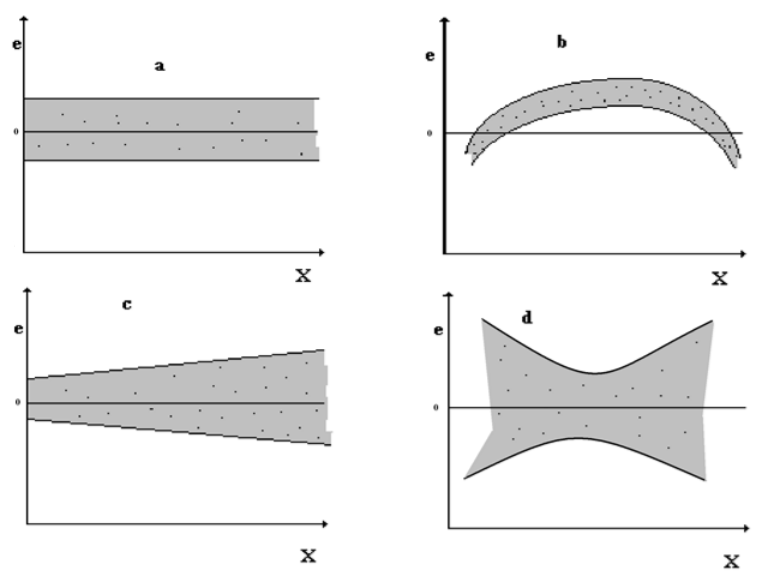
\includegraphics[width=0.5\textwidth]{figures/heteroszkedaszticitas.png} \label{fig:hetero}
\end{figure}

A prediktor változókhoz rendelt \emph{$BETA$ együtthatók} minősítik a változók fontosságát az összefüggésben: minél nagyobb a $BETA$ egüttható abszolútértéke, annál fontosabb a változó. Az együtthatók meghatározása az alábbi összefüggés szerint törénik:

$BETA_i = b_i \cdot \frac{\text{i-dik változó standard szórása}}{\text{célváltozó standard szórása}}$, ahol $b_i$ a regressziós együttható

A meghatározottsági együttható (R-squared) megmutatja, hogy a lineáris regresszióval a célváltozó mekkora hányadát lehet magyarázni. Értéke 0 és 1 között változik, számítása:

$R^2 = \frac{SSR = \Sigma_{i=1}^n\big(\tilde{Y}_i - \bar{Y}  \big)^2}{SSTO = \Sigma_{i=1}^n\big(Y_i - \bar{Y}  \big)^2}$

Az \emph{adjusztált meghatározottsági együttható} segítségével kiküszöbölhetjük azt a problémát, hogy újabb változók bevonásával $R^2$ automatikus nő és túl optimista képet mutat a modell illeszkedéséről. A adjusztált változatban büntetjük a túl sok változó bevonását a modellbe.
%----------------------------------------------------------------------------
\chapter{Faktor- és főkomponensanalízis}


\section{Faktoranalízis}

Nagyszámú, sztochasztikusan erősen összefüggő változónk van, amik redundáns információt hordoznak. A célunk a változók számának csökkentése, de úgy, hogy ezáltal a megfigyelésekben rejlő információ ne csökkenjen lényegesen. Így nehezen megadható fogalmakat definiálhatunk összetett mutatórendszerrel való jellemzés útján. Alapvetően abban különbözik a regresszióanalízistól, hogy a prediktor változók a vizsgálat megkezdésekor nem ismertek, azok előállítása és értelmezése a feladat.

A módszerek általában számolásigényesek és számítógépes programcsomagok segítségével hajthatók végre. Amennyiben többdimenziós normális eloszlásúak a megfigyelések, ezek a módszerek bizonyos optimumtulajdonságokkal rendelkeznek.

A faktoranalízis csak akkor eredményes, ha a vizsgált változók között erős összefüggések vannak. Az összefüggés erejének mérésére több statisztikai is létezik:
\begin{itemize}
\item \emph{Kaiser-Meyer-Olkin statisztika:} változók közötti korrelációs együtthatókkal számol. $0,5$ alatt elfogadhatatlan az összefüggés, $0,9$ fölött csodálatos, a kettő között $0,1$-enként lépeget. A statisztika képlete:

$KMO = \frac{\Sigma_{i=1}^p \Sigma_{j=1, j\neq i}^p R_{ij}^2}{\Sigma_{i=1}^p \Sigma_{j=1, j\neq i}^p \big(\frac{R_{ij}}{\sqrt{R_{ii}\cdot R_{jj}}} \big)^2 + \Sigma_{i=1}^p \Sigma_{j=1, j\neq i}^p R_{ij}^2}$

\item \emph{Minta-alkalmassági érték ($MSA_i$):} megadja, hogy az indulási $p$ változóból melyikeket érdemes elhagyni (amelyeknél az $MSA_i$ érték a legkisebb). A statisztika képlete:

$MSA_i = \frac{\Sigma_{i \neq j} R_{ij}^2}{\Sigma_{i \neq j} \big( \frac{R_{ij}}{\sqrt{R_{ii}\cdot R_{jj}}} \big)^2 + \Sigma_{i \neq j} R_{ij}^2}$, $i = (1,2,...,p)$

\item \emph{Bartlett-féle gömb-próba:} a nullhipotézis, hogy a vizsgált változók függetlenek egymástól. Akkor érdemes továbbmenni, ha ez a próba nem szignifikáns, vagyis a változók között kapcsolat van
\end{itemize}

A $k$-faktoros modellben adottak az $X_1, ..., X_p$ változók, a belőlük alkotott $p$-dimenziós vektor, $\underline{X}$. A vektorról az következő összefüggést tételezzük fel: $\underline{X} = \underline{\underline{A}} \cdot \underline{F} + \underline{U} + \mathbf{E}\underline{X}$, a jelöléseleket a \ref{fig:k-modell}. táblázat mutatja. A faktoranalízist teljesen behatárolja a változók korrelációs mátrixának felépítése. Az átviteli mártixszal pont ezt a korrelációs struktúrát tudjuk feltárni, leírni (adatmátrix $\rightarrow$ korrelációs mátrix $\rightarrow$ átviteli mátrix).

\begin{table}[h]
\centering
\caption{$k$-faktoros modell jelölései} \label{fig:k-modell}
\begin{tabular}{|l|l|}
\hline
Jelölés & Név
\\ \hline
$\underline{\underline{A}}$ & $p$x$k$-s átviteli mátrix
\\ \hline
$\underline{F}$ & $k$-dimenziós közös faktor-vektor
\\ \hline
$\underline{U}$ & $p$-dimenziós egyedi faktor-vektor
\\ \hline
\end{tabular}
\end{table}

A modellel csak akkor érdemes tovább foglalkozni, ha
\begin{itemize}
\item $\underline{F}$ elemei páronként korrelálatlanok, várható értékük 0 és varianciájuk 1,
\item $\underline{U}$ elemei páronként korrelálatlanok, várható értékük 0 és varianciájuk $\Psi_{ii}$ és
\item $\underline{F}$ és $\underline{U}$ elemei páronként korrelálatlanok.
\end{itemize}

Egy $k$-faktoros modell pontosan akkor oldható meg, ha $\underline{X}$ kovariancia mátrixa megegyezik $\underline{\underline{A}} \cdot \underline{\underline{A}}^T +\underline{\underline{\Psi}}$-vel, ahol $\Psi$ $\underline{U}$ kovariancia mátrixa. Ekkor van $p(p+1)/2$ egyenletünk és $p(k+1)$ ismeretlenünk. Amennyiben az egyenletrendszerben kevesebb az egyenlet, mint a változó, különböző kényszerfeltételeket adunk meg, amelyek más-más átviteli mátrixhoz vezetnek. Ezek közül azt választjuk, amelyiknek a legnagyobb a magyarázó ereje.

Az átviteli mátrix együtthatói ($a_{ij}$) jelölik az $X_i$ és $F_j$ közötti kovarianciát, az $\frac{a_{ij}}{\mathbf{D}X_i}$ hányados a közöttük lévő korrelációt adja meg, a $\frac{\Sigma_{j=1}^k a^2_{ij}}{\mathbf{D}^2X_i}$ pedig megadja, hogy a közös faktorok az $i$-dik változó hány \%-át magyarázzák.

A \emph{kommunalitás} ($\mathbf{D}^2X_i = \Sigma_{j=1}^k a^2_{ij} + \mathbf{D}^2U_i$) a változók varianciájának az a része, amit a közös faktorok magyaráznak.

\subsection{Faktorok forgatása}

Az átviteli mátrix egyértelművé tétele segíti a becslési eljárások matematikai elemzését, de az az ára, hogy a kapott közös faktorok nehezen értelmezhetőek. Alkalmas elforgatással esetleg szemléletesebb jelentést tudunk adni a faktoroknak:
\begin{itemize}
\item \emph{Varimax} forgatás esetén azon változók száma kevés lesz, melyekhez sok faktor szerepel nagy súllyal. Célja, hogy minél több 0-hoz közeli faktorsúlyt állítson elő. Ez azért előnyös, mert ha a faktorsúlyok 0-közeliek, akkor a változókat csoportosíthatjuk aszerint, hogy melyik faktor magyarázza őket a legjobban
\item \emph{quartimax} forgatás a magyarázó faktorok számát minimalizálja

\item \emph{equamax} forgatás az előbbi két eljárás keverékét végzi.
\end{itemize}

\section{Főkomponensanalízis}

A főkomponensanalízis a faktoranalízis speciális eset, dimenziószám csökkentésre használható. Az eredetileg $p$ változóval jellemzett statisztikai sokaságot $k<<p$ főkomponenssel jellemzzük úgy, hogy a főkomponensek alapján elvégzett statisztikai elemzések következtetései a $p$-dimenziós sokaságra is érvényesek lesznek. A főkomponensek terében a változók korrelálatlanok lesznek. A főkomponensek korrelálatlanok, csökkenő súlyúak, amiknek az összege a totális variancia; vagyis csökkenő jelentőségűek.

\emph{Watanabe-tétel:} ha $p$ dimenziót lecsökkentünk $k$ dimenzióra, akkor az összes lehetséges dimenziócsökkentési eljárással összevetve a főkomponens analízissel végrehajtott dimenziócsökkentés minimalizálja az információveszteséget.
%----------------------------------------------------------------------------
\chapter{Adatredukciós módszerek}

\section{Klaszteranalízis}

A klaszteranalízis egy adatredukciós módszer, aminek segítségével az eseteket homogén csoportokba sorolhatjuk. A klaszterezés célkitűzése, hogy az "összetartozó" eseteket közös csoportba soroljuk. A hasonlóságot egy $d(\underline{x},\underline{y} )$ távolságfüggvény írja le, melyre igaz, hogy $d(\underline{x},\underline{y}) > 0$, $d(\underline{x},\underline{y})= d(\underline{y},\underline{x} )$ és teljesíti a háromszög-egyenlőtlenséget:
\begin{itemize}
\item Két klaszter távolságát definiálhatjuk a két legközelebbi társ távolságaként, az egymástól legtávolabbi társak távolságaként, vagy a klaszter-középpontok távolságaként
\item Az esetek távolságait is többféleképpen definiálhatjuk: Manhattan-blokkok, Euklideszi távolság, Csebisev ($max_{i=1,...,p} | x_i - y_i|$), stb.
\end{itemize}

A naiv hozzáállás a problémához, ha az összes lehetséges csoportosításból kiválasztjuk a legjobbat. Azonban $N$ elemet $K$ csoportba $\frac{1}{K!}\Sigma_{k=1}^K (-1)^{K-k} {{K}\choose{k}} k^N$-féleképpen lehet sorolni. Ez túl nagy szám. Ehelyett olyan algoritmusok kellenek, amelyek eleve jó csoportosítások képeznek, és ezek közül egy optimum elv segítségével kiválasztható egy nagyon jó.

A \emph{k-közép} módszer olyan klaszterező eljárás, amikor előre meg kell adni a klaszterek számát. Lépéseit \emph{McQueen-tételként} ismerjük: válasszuk ki a klaszterek számát ($k$). Véletlenszerűen hozzunk létre $k$ számú klasztert és határozzuk meg minden klaszter közepét (vagy válasszunk $k$ véletlen klaszter-középpontot).
Az esetvektorok a legközelebbi klaszter-középponthoz lesznek rendelve. Számoljuk ki az új klaszter-középpontokat! Az előzőeket isméterljük, amíg valamilyen konvergencia kritérium nem teljesül. Előnye, hogy nagy esetszámú adatmátrix is feldolgozható vele, egyszerű, gyors és végessor lépésben leáll. Hátránya, hogy a metrika beépített (Euklideszi), körülményes a koordinátázás, előre meg kell adni a klaszterek számát és az eredmény függ a sorrendtől.  A k-közép algoritmus általánosítása a \emph{k-medoids}, ami tetszőleges metrikával működik.

A \emph{hierarchikus klaszterezés} egyelemű klaszterekből indul ki és minden lépésben a két legközelebb fekvő klasztert összevonva csökkenti a klaszterek számát, amíg egyetlen klaszterbe nem kerül minden eset. A folyamatot dendogrammon követhetjük végig és azt a köztes állapotot fogadjuk el, amikor az összevont klaszterek elég távol voltak egymástól. Előnye, hogy nem kell előre tudni a klaszterek számát, ráadásul változtatható a távolság- és hasonlósági-mérték. Hátránya, hogy csak kis dimenziószám esetén indítható el.

\section{Diszkriminanciaanalízis}

Diszkriminanciaanalízis segítségével az esetek egy kategóriaváltozó értékei alapján osztályokba vannak tagolva. A feladat az, hogy a többdimenziós térben az osztályokat szeparáló felületekkel elválasszuk. A szeparációs felületek az eseteket vagy objektumok jellemző változók alkalmas lineáris kombinációi. A módszerrel újabb objektumok csoportokhoz tartozásának lehető legjobb előrejelzését is megadhatjuk.

\emph{Csoportképző változó:} természetes számokkal kódolt kisszámú értéket vehet fel, amelyek egymást kölcsönösen kizáró kategóriáknak felelnek meg.

\emph{Prediktor változó:} többdimenziós, normális eloszlású kvantitatív adatokat kell tartalmaznia minden csoportban közel azonos kovariancia mátrixokkal.

\emph{Diszkriminancia-függvény:} a csoportképző változók alkalmas módon megválasztott lineáris kombinációja, amelynek alapján a csoporthoz tartozás megadható. A lineáris kombináció konstansait úgy választjuk meg, hogy a $\frac{\Sigma_i (\bar{x}_i - \bar{x})^2}{\Sigma_j \Sigma_i (x_{ij} - \bar{x}_i)^2}$ hányados értéke maximális legyen.

\section{Osztályozás}

Osztályozásról beszélünk, ha ismert kategóriájú esetek segítségével (tananyag) döntésfüggvényt konstruálunk, amivel ismeretlen kategóriájú esetekben is tudunk osztályokat rendelni. A $\mathcal{D}_n = \{ (X_1,Y_1), ..., (X_n,Y_n)\}$ halmazt \emph{tananyagnak} nevezzük. $X_i$ az $i$-dik tanulópont, a belőlük képzett halmaz pedig a tanulópont-halmaz. $Y_i$ a megfelelő tanítás. Az osztályozás folyamata 3 lépésből áll:
\begin{enumerate}
\item A tananyag előfeldolgozása: csak egyszer kell elvégezni, míg az osztályozást nagyon sokszor. Az előfeldolgozás költsége megtérül, ha kisebb költséggel osztályzunk.
\begin{itemize}
\item Ritkítás: részhalmaz előállítása, ami pontosan osztályozza a tananyagot és minimális elemszámú
\item Tömörítés: olyan tananyag készítése, ami kevesebb elemből áll, mint az eredeti és pontosan osztályozza azt
\item Átdefiniálás: megadunk egy transzformációt, ami átdefiniálja az osztályokat, ezzel új tananyagot készíthetünk
\item Szűrés: olyan részhalmazt akarunk előállítani, amelynél a tananyag pontjait a legközelebbi szomszék módszerrel pontosabban lehet osztályozni
\end{itemize}
\item A döntésfüggvény előállítása a $\mathcal{D}_n$ tananyag függvényeként
\item Ismeretlen alakzatvektorok osztályozása
\end{enumerate}

A \emph{legközelebbi társ módszerével} minden osztályozandó pontot abba az osztályba fogunk sorolni, amelyik osztálynak a már létező tagjai közül valamelyikre az osztályozandó pont a legjobban hasonlít. A hasonlóságot itt is egy távolságfüggvény írja le. Alapesetben ez $n$ db távolság kiszámítását jelenti, vagyis jó lenne gyorsítani az algoritmust. A gyorsításhoz szükség van a tananyag előfeldolgozásából nyert adatokra, statisztikákra. A gyorsítás ún. \emph{kizárási feltételek} alapján történik, amik megadják, hogy mikor biztosan nem legközelebbi szomszédja egy tanulópont egy adott esetnek, pl. adott esettől vett távolsága nagyobb, mint a legkisebb távolság kétszerese; van olyan tanulópont, amitől több, mint kétszer távolabb van, mint a potenciális szomszéd.

%----------------------------------------------------------------------------
\chapter{Többdimenziós skálázás (MDS)}

Adott egy olyan adatállomány, amelyet valamilyen megadott külső objektumokra vonatkozó hasonlósági vagy különbözőségi adatok (ált. skálázott szubjektív vélemények vagy észlelt különbségek) alkotnak. A cél olyan geometriai reprezentációk létrehozása a hasonlósági vagy különbözőségi adatokból, amelyek az adott külső tárgy (észlelt) viszonyát egy megfelelő dimenzió-számú geometrikai térben a lehető legpontosabban tükrözik vissza. Az eljárás eredménye mindig egy ponthalmaz egy adott dimenziószámú geometriai térben. A ponthalmaz képe alapján kísérletet tehetünk koordinátatengelyek megadására, amivel rejtett dimenziókat tárhatunk fel. Pl. milyen szempontokat tartanak fontosnak az emberek autóvásárlásnál? Miért szavaznak arra a politikusra, amelyikre?

Sokszor már a szemléletes ábrázolás önmagában is sokat segít az adott jelenség megértésében, ha van benne valamilyen szabályszerűség. Azonban az ábrázolás önmagában még nem skálázás. Ha a térben sikerül olyan koordináta tengelyeket találni, amelyek mentén az objektumok elhelyezkedése jól értelmezhető, akkor ezeknek a \emph{tengelyeknek} az alkalmas \emph{beskálázásával} minden objektumhoz skálaértékeket rendelhetünk az adott dimenziók mentén.

Azonban az érzékelt különbözőségeknek pontosan megfelelő geometriai konfiguráció nem mindig állítható elő, a feladatnak nem mindig létezik egzakt megoldása az adott térben. Azért a cél az, hogy legalább a lehetséges legjobb közelítő megoldást (optimális konfigurációt) találjuk meg.

Az MDS alkalmazásához speciálisabb távolság vagy hasonlóság jellegű adatokra van szükség, amelyek általában csak erre a célra tervezett kísérletekban vagy felmérésekben nyerhetők. Amennyiben viszont sikerül alkalmas hasonlósági mértékeket definiálni és azokat megfelelő pontossággal mérni, akkor az MDS lényegesen jobb eredményt ad a faktoranalízisnél.

\section{Metrikus klasszikus MDS}

A \emph{klasszikus MDS (CMDS)} modellje csupán egyetlen különbözőségi mátrixot képes egyidejűleg kezelni és megkívánja a bemenő adatoktól a legalább intervallum-skálát. Alkalmazhatósága korlátozott, mert tipikusan több személy adatait szeretnénk egyidejűleg feldolgozni. Az $i$ és $j$ pontoknak megfelelő objektumok közötti különbözőség-érzékletet a létrehozott pontkonfigurációban a pontok euklideszi távolságával képezi le. A $\underline{\underline{D}}$ távolság-mártix elemei az egyes távolságértékek, amelyek a pontkonfigurációt jellemzik. Ennek a konfigurációnak az eltérése az eredeti észlelési adatokat tartalmazó $S$ különbözőség-mátrixtól mutatja, hogy egy megtalált megoldásnak mekkora a hibája. A illeszkedést a következő mutatók segítségével tudjuk mérni:
\begin{itemize}
\item \emph{S-stress:} $\sqrt{\frac{\text{hibamátrix (E) elemei négyzeteinek összege}}{\text{S-ből alkalmas lineáris transzformációval képzett mátrix (T) elemei négyzeteinek összege}}}$,\\szemléletesen a modell által meghatározott térben az összes észlelt különbözőséghez képest mekkora az eltérés az elméleti távolságok és a pontkonfigurációban létrejött távolságok között. Ha tökéletes a megfelelés, értéke 0
\item \emph{Stress:} mint az s-stress, csak nem távolságnégyzetekkel, hanem magukkal a távolságokkal számol
\item \emph{RSQ:} $D$ és $T$ megfelelő elemei között kiszámított korrelációs együttható négyzete.
\end{itemize}
A rekonstrukció akkor elfogadható, ha az s-stress és a stress értékei 0,20 alatt vannak (0,05 alatt kíváló). RSQ-nál a kisebb értékek rosszabb illeszkedést jeleznek.

Metrikus CMDS esetén probléma, hogy nincs garancia arra, hogy az emberek hasonlósági ítéleteiket valóban egyenletesen skálázzák, ráadásul egyesek kifejezetten sarkítják a véleményüket. A gyakorlatban ráadásul inkább csak ordinális skálájú adataink vannak, nem intervallum-skálájúak. Megoldás: nemmetrikus MDS!

\section{Nemmetrikus CMDS}

\emph{Nemmetrikus MDS} esetén a távolságokat rangszámokkal helyettesítjük, amik az eredeti távolságok sorrendjét reprezentálják. Ábrázolásnál a rangszámok a pontok köré rajzolt kör/gömb/stb. sugarának felelnek meg. Ekkor azonban a konfiguráció instabil: az egyes pontok helye megváltoztatható anélkül, hogy a rangsor megváltozna. Azonban a pontok számának növelésével az egyes pontok mozgástere radikálisan szűkül. A három illeszkedési mutató ugyanúgy használható itt is, mint metrikus esetben, csak $T$-t nem lineáris, hanem monoton transzformációval kell létrehozni.

\section{Továbbfejlesztett MDS modellek}

Több kísérleti személy eredményeinek együttes kiértékelése az előző módszerekkel problémás, mert csak egyetlen különbözőség-mátrixot tudnak egyidőben használni. A CMDS egyszerű személyenkénti ismételgetése azonban általában nem elfogadható, mert közvetve feltételei, hogy az egyes személyek különbözőség-érzékletei  egymástól függetlenek, nincs bennük semmi közös. Az igazán jól használható megoldásokhoz más típusú matematikai modellekre volt szükség, pl.
\begin{itemize}
\item Replicated MDS: ez már több különbözőségi mátrixot is képes egyidejűleg kezelni és feltételezi, hogy az egyes objektumok különbözőségei bizonyos véletlenszerű hibáktól eltekintve azonos mértékben tükröződnek $\rightarrow$ az adatmátrixok egymás replikái
\item Weighted MDS: több különbözőségi mátrixot is képes egyidejűleg kezelni és a válaszok mögött meghúzódó egyéni észlelési és kognitív folyamatok különbségeiről is bizonyos információkat tud adni
\end{itemize} 

%----------------------------------------------------------------------------
\chapter{Kérdőíves felmérések módszertana}

A kérdőívnek alapvetően kétféle tétele van: kérdések és állítások. A kérdő és a kijelentő forma egyaránt hasznos lehet, kombinálásukkal elkerülhető a monotómia.
\begin{itemize}
\item \emph{Kérdések:} a kérdések sorrendje hatással lehet a későbbi válaszokra, ezért az általánostól érdemes indulni a konkrét felé és témakörönként csoportosítani kell őket. Önkitöltős tesztnél fontos az is, hogy előbb érdekes kérdések jöjjenek, különben a kérdezett elunja magát és a kérdőív nagy részét nem tölti ki. A kérdések sorrendjének randomizálása megnehezítheti a kitöltést, ezért előre fel kell mérni, hogy melyik kérdés vezetheti meg a kérdezettet egy később felteendő kérdésnél. Ha van ilyen, azt hátrébb kell sorolni
	\begin{itemize}
	\item A kérdések legyenek egyértelműek, világosak, csak egy dologra kérdezzenek rá, relevánsak legyenek és ne sugalmazzák a választ
	\item A kérdezettnek kompetensnek kell(ene) lennie és hajlandónak válaszolni
	\item \emph{Nyitott kérdés:} a válaszoló a saját szavaival fogalmazza meg a választ. A nyitott kérdések előnye, hogy nem köti meg a kérdezett fantáziáját, viszont nehezen kódolható, ráadásul teret ad a kutató szabad értelmezésének, amit torzítást eredményezhet. Előfordul, hog a válasz irreleváns
	\item Zárt kérdések esetében a válaszolónak egy listából kell kiválasztania a lehetséges válaszokat. Fontos, hogy a válaszok teljes eseményrendszert alkossanak. A zárt kérdéseket könnyen és egyértelműen lehet kódolni számítógépes feldolgozáshoz, de figyelni kell a hiányzó válaszok feldolgozásánál. Zárt kérdéseknél előfordulhat, hogy a kérdezett több választ is meg tudna jelölni, ráadásul a gyűtő válasz ("egyéb") nagyon tág lehet
	\item \emph{Feltételes kérdések:} elágazási pontok a kapott választól föggően
	\item \emph{Mátrix kérdések:} ha egy csoportban teszünk fel zárt kérdéseket Likert-skálás válaszokkal, mátrix struktúrát alkalmazhatunk (táblázatos forma: sorok a kérdések, oszlopok a lehetséges válaszok)
	\end{itemize}
\item \emph{Állítások:} akkor alkalmazzuk, ha a kutató azt akarja megtudni, hogy milyen mértékben oszt a kérdezett bizonyos attitűdöt vagy nézetet. Az attitűdöt egy tömör kijelentésben összefoglaljuk, és megkérdezzük, mennyiben ért ezzel egyet a kérdezett.
\end{itemize}

A lehetséges válaszokat Likert formalizálta, megalkotva a \emph{Likert-skálát}. Likert-skála esetén a válaszolónak egy állítással való egyetértés mértékét, vagy egy vélemény helyeslését kell kifejeznie.  A kérdőívszerkesztőnek csak az állítást kell meghatároznia, maga a skála mindig ugyanaz, pl. Egyetért - Közömbös - Nem ért egyet. A skála lehetnek
\begin{itemize}
\item Verbális/nem verbális
\item Egyirányú: pl. 5 = teljes mértékben egyetért, ..., 1 = egyáltalán nem ért egyet
\item Középre rendezett: pl. 5 = teljesen elégedett, ..., 3 = közömbös, ... 1= teljesen elégedett
\item Szemantikus differenciál: az intenzitást és a tartalmat egyszerre vizsgálja a megkérdezett gondolkodásmódjában egy hétfokozatú skálán, pl. korszerű 1,2,...,6,7 régimódi. Így egyéni és csoportátlagok, szóródások számíthatók
\end{itemize}
A skálaértékek között egyenletes távolságoknak kell lenniük, biztosítani kell a megfelelő szórást és szemantikus differenciál esetén a verbális végpontoknak tartalmilag szembenállóknak kell lenniük

\emph{Primer adatok:} a mintavételből nyert adatok.

\emph{Szekunder adatok:} meglévő adatázisokból, releváns forrásokból és a szakirodalomból nyert adatok.

\section{Adatgyűjtési technikák}

\emph{Interjú módszer:} az interjú módszer korlátozza a kutató előítéletéből fakadó korlátokat, interaktív és lehetőséget ad a változtatásra. Személyesen vagy telefonon történik jegyzeteléssel vagy hangrögzítéssel. Lehet:
\begin{itemize}
\item Strukturálatlan: szabad beszélgetés (nehéz a kódolása)
\item Dinamikus, non-direktív: ilyen csak irányító kérdések vannak, a kérdezőnek nem szabad közbekérdezni
\item Strukturált: irányított beszélgetés, ami kódolható és statisztikai feldolgozásra alkalmas
\end{itemize}

\emph{Kérdőíves adatgyűjtés:} sikere a kérdések megfogalmazásán áll vagy bukik. Kutatási kérdések megválaszolását szolgálja, a válaszok alapján kell tudni dönteni a hipotézisről. Lépései:
\begin{enumerate}
\item Kérdőív-szerkesztés: ne legyen túl rövid, elrendezésnél fekvő és álló is elfogadható, legyen rajta verziószám és a papírnak csak az egyik oldalára nyomtassunk. A kérdéseket és válaszokat számozzuk, az utasításokat CSUPA NAGY BETŰVEL ÍRJUK. Ha 5 vagy kevesebb választási lehetőség van egy zárt kérdésnél, akkor azokat két függőleges oszlopba kell rendezni, kerüljük a tagadó kérdéseket, negatív megfogalmazást
\item Kérdőív tesztelése
\item Mintavétel (lásd \ref{ch:mintavetel}. tétel)
\item Adatgyűjtés: lehet személyes megkérdezés, telefonos felvétel vagy önkitöltős kérdőív, lehetőség van másodelemzésekre. Pl. önkitöltő kérdőív fókuszcsoportban (célcsoport közös beszélgetésen vesz rész, ált. 8 főből áll), vezetőknél kitöltött kérdezőbiztosi, kombinált telefon/posta, stb.
\item Kiértékelés
\end{enumerate}

%----------------------------------------------------------------------------
\chapter{Mintavételezés} \label{ch:mintavetel}

A statisztika célja a halmaz egészének kevés adattal történő tömör 
jellemzése, és a populáció egyedeinek leírására bevezetett változók közötti kapcsolatok leírása. Arra nincs lehetőség (erőforrás), hogy  a populációminden egyes eleméről adatokat szerezzünk be, azaz mintát kell vételeznünk a sokaságból.

\emph{Minta:} A sokaság elemeinek egy csoportja. A mintajellemzőkből (statisztikákból) tudunk valamilyen következtetést levonni a teljes sokaságra.

\emph{Reprezentativitás:} nem reprezentatív mintából levont következtetések értékelhetetlenek, torzak. Az alkalmazott statisztikai módszerek, becslési hibák akkor lesznek érvényesek, ha a minta, amivel számolunk reprezentatív! A populáció minden egyes elemének ugyanakkora esélyt kell biztosítani a mintába kerüléshez. A minta elemszámának elég nagynak kell lennie ahhoz, hogy a következtetéseink átvihetők lehessenek a populációra is. A szükségesnél ne kelljen nagyobb mintát feldolgozni, mert az költségesebb.

\emph{Mintavételi keret:} a mintavételi egységekről (vizsgálati egység, amelyik rendelkezik a keresett információval, vagy az az alapegység, amelyik magában foglalja a sokaság elemeit) készült felsorolás, amely segítségével azonosíthatóak az elemek. Amennyiben a populáció bizonytalanul körülhatárolható csak, a mintavételi keretet keressük meg, amely alkalmas arra, hogy a populáció minden egyes elemét azonosítsuk és bevonjuk bármely mintánkba.

\section{Mintavételezési technikák}

\emph{Cenzus:} A sokaság elemeinek teljes számbavétele. Cenzust alkamazunk, ha kicsi a sokaság, figyelni kell az egyedi esetekre, sok idő és pénz áll rendelkezésre vagy nagon szóródik a megfigyelt jellemző a sokaságban.

\emph{Visszatevéses mintavétel:} egy adott elem elvileg többször is a mintába kerülhet.

\emph{Visszatevés nélküli mintavétel:} egy elem csak egyszer kerülhet a mintába.

\emph{Bayes-technika:} minden egyes kiválasztást követően kiszámítják a mintajellemzésőket és meghatározzák a költségeket, és ezek alapján válsztják a következő egyedet.

\emph{Nem véletlen mintavételi technikák:} a ilyen technikák esetében nem minden esetben teljesül a reprezentativitás. Azonban feltáró kutatáshoz jól használható, illetve alkalmazzuk, ha nagyok a nem mintavételi hibák, a sokság homogén, vagy nem statisztikai módszerekkel kívánjuk elemezni a mintát.
\begin{itemize}
\item Önkényes mintavétel: a minta elemeit általában kérdezőbiztos választja ki, nincs mintavételi keret, amiből választani lehetne. Olcsó, a mintavételi egységek könnyen elérhetők, de semmilyen meghatározható sokaságot nem reprezentálnak és semmilyen általánosításra nem ad módot. Mire jó: leíró kutatások, hipotézisek felállítása
\item Elbírálásos mintavétel: a kutató saját tapasztalatai alapján választ a sokaság elemei közül és eldönti, hogy bekerüljenek-e a mintába, vagy sem. Pl. teszthelyszínek kiválasztása, szakértők kiválasztása, stb.
\item Kvótás mintavétel: A kutató felállítja a sokaság kontroll kategóriáit, azaz a kvótákat, a mintaelemeket a kvótának megfelelően önkényesen vagy elbírálással választja ki. Ha kimarad a sokaság egy fontos jellemzője, akkor a minta nem reprezentatív
\item Hólabda mintavétel: egyvalakit, vagy egy kis csoportot megkeresünk és a kezdeti csoport tagjait arra kérjük, hogy ajánljanak másokat, akik szintén a célsokasághoz tartoznak. Akkor használjuk, ha speciális jellemzővel bíró sokaságot keresünk.
\end{itemize}

\emph{Véletlen mintavételi technikák:} az elérendő cél az, hogy 
a minta jellemzői teljes egészében megegyezzenek a célsokaság jellemzőivel, azaz ne legyen torzítás. Ha mégis lenne eltérés, akkor a különbség legyen statisztikailag mérhető. Az így vett minták jellemzői kivetíthetők az egész sokaságra. Használjuk leíró kutatásokhoz, ha nagyok a mintavételi hibák vagy a sokaság szórása nagy és statisztikai módszerekkel kívánjuk elemezni a mintát.
\begin{itemize}
\item Egyszerű véletlen mintavétel: a sokaság minden eleme ismert és azonos valószínűséggel kerülhet be a mintába. Minden elemet egymástól függetlenül, a mintavételi keretből véletlen eljárással választunk ki
\item Szisztematikus mintavétel: a mintavételi keretben véletlenszerűen kijelölnek egy kezdőpontot, majd kiválasztják a mintavételi keret $i$-dik elemét, $i = [N/n]$, ahol $N$ a mintavételi keret elemszáma, $n$ pedig a minta elvárt nagysága. Akkor működik jól, ha nincsenek sorbaállítva az egyedek a vizsgált jellemzővel összefüggésben
\item Rétegzett mintavétel: sokaságot csoportokra bontják valamilyen ismert rétegképző ismérv segítségével, az egyes rétegekből pedig egyszerű véletlen mintavétellel választanak. Attól függően, hogy a rétegekből kiválasztott elemek száma arányos-e a rétegnek a teljes sokasághoz viszonyított nagyságával, beszélhetünk arányos és nem arányos rétegezésről
\item Csoportos mintavétel: A célsokaságot egymást kölcsönösen kizáró csoportokra bontják, amelyek együttesen lefedik az egész sokaságot (statisztikai populációt). Az így képzett csoportokból egyszerű véletlen mintát vesznek (csoportokat választanak ki). A kiválasztott csoportból vagy mindenki kiválasztanak, vagy csoporton belül egyszerű véletlen mintavételeznek.
\item Többlépcsős mintavételezés: nagyobb egységeket részekre bontjuk és a részek között véletlenszerűen választunk egyet. A kiválasztott rész újabb részekre bontjuk és véletlenszerűen megint választunk...
\item Szekvenciális mintavétel: a sokaság elemeiből egymást követően veszünk mintát, majd valamilyen mintavételt követően elvégezzük az elemzést és eldöntjük, hogy kell-e újabb elemet választani
\item Kettős mintavétel: a sokaság elemeiből kétszer veszünk mintát
\end{itemize}

\section{A szükséges minta elemszám meghatározása}

Minél pontosabb információra van szükség, annál nagyobb mintát kell venni. Ám minél jobban nő a minta, annál kisebb a javulás a mintanagyság egységnyi növekedésével. Léteznek ökölszabályok és tudományos módszerek is az elemszám meghatározására

Ökölszabály: kis csoport (elemszám max. 30-35) esetén a teljesen populációt be kell venni a mintába, vagyis cenzust kell alkalmazni. Nagyobb elemszám esetén a minta elemszáma és a teljes populáció között közel logaritmikus kapcsolat áll fenn.

Tudományos módszerek: minimális mintaelemszám meghatározásakor a \\$\mathbf{P}\big( | \bar{x}_n - m | \leq \epsilon \big)\geq 1-\mu$ relációra keressük a megfelelő $n$-eket. A reláció jelentése: mekkora $n$ elemszám garantálja, hogy a mintaátlag a minta várható értékétől legfeljebb $\epsilon$ távolságra esik $1-\mu$ valószínűséggel? Ha a 3 paraméter ($n$, $\epsilon$, $\mu$) bármelyik kettőt ismerjük, akkor alsó-becslést tudunk adni a harmadikra.
\begin{itemize}
\item Egymintás t-próbához (centrális határeloszlás-tétel alapján): ahhoz, hogy $(1-\alpha)$ valószínűséggel kimutassunk egy legalább $2d$ nagyságű különbséget, a mintának $\frac{u_{\alpha/2}^2 \cdot \sigma^2}{d^2}$ elemet kell tartalmaznia. $u_{\alpha/2}^2$ a standard normális eloszlás $\alpha/2$ valószínűséghez tartozó értéke, $\sigma$ az elméleti szórás vagy annak becslése, $d$ pedig a konfidencia intervallum szélességének fele
\item Kétmintás t-próbához Beyer készített táblázatot figyelembe véve a másodfajú hibát és hogy milyen valószínűséggel szeretnénk a különséget kimutatni
\item Paraméteres módszerek:
	\begin{itemize}
	\item ismert $\sigma$ szórás esetén: $n \geq \frac{z_{\mu/2}^2 \cdot \sigma^2}{\epsilon^2}$, ahol $\Phi(z_{\mu/2}) = 1- \mu/2$
	\item ismeretlen szórás esetén:  $n \geq \frac{t_{\mu/2}^2 \cdot s_n^2}{\epsilon^2}$, ahol $F_{n-1}(t_{\mu/2}) = 1- \mu/2$ és $s_n^2$ a minta szórásnégyzete
	\end{itemize}
\item Ha a mérések garantáltan az $(a,b)$ intervallumba esnek
	\begin{itemize}
	\item ismeretlen szórás esetén Hoeffding-egyenlőtlenség: $n \geq -\frac{ln(\mu/2) \cdot \frac{(b-a)^2}{2}}{\epsilon^2}$
	\item ismert $\sigma$ szórás esetán Bernstein-egyenlőtlenség: $n \geq -\frac{ln(\mu/2) \cdot (2 \sigma^2 + 2\epsilon \frac{b-a}{3})}{\epsilon^2}$
	\end{itemize}
\item Csernov-egyenlőtlenség
\end{itemize}

%\listoffigures\addcontentsline{toc}{chapter}{Ábrák jegyzéke}
%\listoftables\addcontentsline{toc}{chapter}{Táblázatok jegyzéke}

%\bibliography{mybib}
%\addcontentsline{toc}{chapter}{Irodalomjegyzék}
%\bibliographystyle{plain}

\include{appendices}

\label{page:last}
\end{document}
